% documentclass options:
\documentclass[11pt,
  a4paper,
  parskip=half, % This is some extra vertical space between paragraphs, the suggestion is 2cm which is ugly, so we use what the script gives us
  % You can also set it to full for even more space. But there is a bad tex style decision: Parskip also changes the spacing between list items such as
  % enumerate and itemize. So we include the enum item package and set itemsep=.5em, of course you can change this
  BCOR=10mm, % BCOR is a binding correction
  English,
  % If you'd rather have a one-sided thesis, add `Oneside' to the document class
  % Oneside,
  % Ngerman is needed for hyphenation if the thesis contains parts written in German, switch order with English if you write mainly in English.
  % Remember to change the order in the babel package (below) as well.
  % Last language is the preferred one.
  ngerman]{scrbook}
\usepackage[english, ngerman]{babel} % If you write mainly in English change order to ngerman, english. Also, change that in the document class options above.
% Include of titling must happen before \title etc.
% That's why it's not in setup.tex
\usepackage{titling}
% define location for all figures


\title{Model Predictive Control for trajectory following Automated Guided Vehicles}
\author{Akash John Subash}

% Change to your first examiner
% The ~ enables non-sentence spacing after a period
\newcommand{\firstexaminer}{Prof.~Dr.~Moritz Diehl}
% Change to your second examiner
\newcommand{\secondexaminer}{Prof.~Dr. Abhinav Valada}
% Change to your advisers
\newcommand{\advisers}{Daniel Klöser, Jonathan Frey}

% include all packages and define commands in setup.tex

%------------------------------------------------------------------------------
%       package includes
%------------------------------------------------------------------------------
    % font encoding is set up for pdflatex, for other environments see
    % http://tex.stackexchange.com/questions/44694/fontenc-vs-inputenc
    \usepackage[T1]{fontenc}  % 8-bit fonts, improves handling of hyphenations
    \usepackage[utf8x]{inputenc}
    % provides `old' commands for table of contents. Eases the ability to switch
    % between book and scrbook
    \usepackage{scrhack}
    \usepackage{upgreek}
    \usepackage[euler]{textgreek}
    \usepackage{needspace}
    % \usepackage{hyperref}
    % \usepackage[options]{natbib}
    % \usepackage{biblatex}
    % \addbibresource{./syscop_bibtex/thesis.bib}    
    % ------------------- layout, default -------------------
    % adjust the style of float's captions, separated from text to improve readabilty
    \usepackage[labelfont=bf, labelsep=colon, format=hang, textfont=singlespacing]{caption}
    % With format = hang your caption will look like this:
    % Figure 1: Lorem ipsum dolor sit amet,
    %           consectetuer adipiscing elit.
    %           Ut purus elit, vestibulum
    % If you instead want
    % Figure 1: Lorem ipsum dolor sit amet,
    % consectetuer adipiscing elit. Ut purus
    % elit, vestibulum
    % change to format=plain
    \usepackage{chngcntr}  % continuous numbering of figures/tables over chapters
    \counterwithout{equation}{chapter}
    \counterwithout{figure}{chapter}
    \counterwithout{table}{chapter}

    % Uncomment the following line if you switch from scrbook to book
    % and comment the setkomafont line
    %\usepackage{titlesec}  % remove "Chapter" from the chapter title
    %\titleformat{\chapter}[hang]{\bfseries\huge}{\thechapter}{2pc}{\huge}
    \setkomafont{chapter}{\normalfont\bfseries\huge}

    \usepackage{setspace}  % Line spacing
    \onehalfspacing
    % \doublespacing  % uncomment for double spacing, e.g. for annotations in correction

    % ------------------- functional, default-------------------
    \usepackage[dvipsnames]{xcolor}  % more colors
    \usepackage{array}  % custom format per column in table - needed on the title page
    \usepackage{graphicx}  % include graphics
    \usepackage{svg}
    \usepackage{subfig}  % divide figure, e.g. 1(a), 1(b)...
    \usepackage{amsmath}  % |
    \usepackage{amsthm}   % | math, bmatrix etc
    \usepackage{amsfonts} % |
    \usepackage{calc}  % calculate within LaTeX
    \usepackage[unicode=true,bookmarks=true,bookmarksnumbered=true,
                bookmarksopen=true,bookmarksopenlevel=1,breaklinks=false,
                pdfborder={0 0 0},backref=false,colorlinks=false]{hyperref}
    \usepackage{etoolbox} % if-else commands


    %==========================================
    % You might not need the following packages, I only included them as they
    % are needed for the example floats
    % ------------------- functional, custom -------------------
    \usepackage{algorithm,algpseudocode}
    \usepackage{bm}  % bold greek variables (boldmath)
    \usepackage{tikz}
    \usetikzlibrary{positioning}  % use: above left of, etc
    
    % required for the ToDo list
    \usepackage{ifthen}

    % Improves general appearance of the text
    \usepackage[protrusion=true,expansion=true, kerning]{microtype}
    \usepackage{enumitem}
    % nicer font for pdf rendering
    %\usepackage{lmodern}
    
    % For nicer looking tables
    \usepackage{booktabs}

    % usually you don't need this, just for demonstration of a longer caption
    \usepackage{lipsum}
    \usepackage{acronym}
%------------------------------------------------------------------------------
%       (re)new commands / settings
%------------------------------------------------------------------------------
    % ----------------- referencing ----------------
    \newcommand{\secref}[1]{Section~\ref{#1}}
    \newcommand{\chapref}[1]{Chapter~\ref{#1}}
    \renewcommand{\eqref}[1]{Equation~(\ref{#1})}
    \newcommand{\figref}[1]{Figure~\ref{#1}}
    \newcommand{\tabref}[1]{Table~\ref{#1}}

    % ------------------- colors -------------------
    \definecolor{darkgreen}{rgb}{0.0, 0.5, 0.0}
    % Colors of the Albert Ludwigs University as in
    % https://www.zuv.uni-freiburg.de/service/cd/cd-manual/farbwelt
    \definecolor{UniBlue}{RGB}{0, 74, 153}
    \definecolor{UniRed}{RGB}{193, 0, 42}
    \definecolor{UniGrey}{RGB}{154, 155, 156}


    % ------------------- layout -------------------
    % prevents floating objects from being placed ahead of their section
    \let\mySection\section\renewcommand{\section}{\suppressfloats[t]\mySection}
    \let\mySubSection\subsection\renewcommand{\subsection}{\suppressfloats[t]\mySubSection}



    % ------------------- math formatting commands -------------------
    % define vectors to be bold instead of using an arrow
    \renewcommand{\vec}[1]{\mathbf{#1}}
    \newcommand{\mat}[1]{\mathbf{#1}}
    % tag equation with name
    \newcommand{\eqname}[1]{\tag*{#1}}
    % \usepackage{newunicodechar}
    % \newunicodechar{^^^^2502}{|}

    % ------------------- pdf settings -------------------
    % ADAPT THIS
    \hypersetup{pdftitle={\thetitle},
                pdfauthor={\theauthor},
                pdfsubject={Undergraduate thesis at the Albert Ludwig University of Freiburg},
                pdfkeywords={deep learning, awesome algorithm,  undergraduate thesis},
                pdfpagelayout=OneColumn, pdfnewwindow=true, pdfstartview=XYZ, plainpages=false}


    %==========================================
    % You might not need the following commands, I only included them as they
    % are needed for the example floats

    % ------------------- Tikz styles -------------------
    \tikzset{>=latex}  % arrow style


    % ------------------- algorithm ---------------------
    % Command to align comments in algorithm
    \newcommand{\alignedComment}[1]{\Comment{\parbox[t]{.35\linewidth}{#1}}}
    % define a foreach command in algorithms
    \algnewcommand\algorithmicforeach{\textbf{foreach}}
    \algdef{S}[FOR]{ForEach}[1]{\algorithmicforeach\ #1\ \algorithmicdo}

    % line spacing should be 1.5
    \renewcommand{\baselinestretch}{1.5}

    % set distance between items in a list, for more details see the
    % enumitem package: https://www.ctan.org/pkg/enumitem
    \setlist{itemsep=.5em}
    
    % use ra in your tables to increase the space between rows
    % 1.3 should be fine
    \newcommand{\ra}[1]{\renewcommand{\arraystretch}{#1}}

	% ToDo counters
	\usepackage{ifthen} %für whiledo-Schleife
	\newcounter{todos}
	\setcounter{todos}{0}
	\newcounter{extends}
	\setcounter{extends}{0}
	\newcounter{drafts}
	\setcounter{drafts}{0}

	% ------------------- marker commands -------------------
    % ToDo command
    \newcommand{\todo}[1]{\textbf{\textcolor{red}{(TODO: #1)}}\refstepcounter{todos}\label{todo \thetodos}}
	\newcommand{\extend}[1]{\textbf{\textcolor{darkgreen}{(EXTEND: #1)}}\refstepcounter{extends}\label{extend \theextends}}
	% Lighter color to note down quick drafts
	\newcommand{\draft}[1]{\textbf{\textcolor{NavyBlue}{(DRAFT: #1)}}\refstepcounter{drafts}\label{draft \thedrafts}}
	
	% microtype with lmodern, see https://tex.stackexchange.com/questions/75305/microtype-warning-with-lmodern-package-and-koma-script
	%\DeclareMicrotypeAlias{lmss}{cmr}
	
	%% SYSCOP specific packages
	\usepackage{optidef}
	
	%% useful commands - Jonathan Frey
	\newcommand{\nz}{{n_{\text{z}}}}
	\newcommand{\R}{{\mathbb{R}}}
	\newcommand{\Co}{{\mathbb{C}}}
	\newcommand{\tran}{^\top}
	
	\newcommand{\ind}[1]{{_{\textrm{\normalfont#1}}}}
	\newcommand{\diag}[1]{\text{\normalfont diag}\left( {#1} \right)}
	\newcommand{\upind}[1]{\ensuremath{{^{\textrm{\normalfont#1}}}}}
	
	\newcommand{\quot}[1]{``{#1}''}
	\newcommand{\code}[1]{\texttt{#1}}
	\newcommand{\Set}[2]{\{\, #1 \mid #2 \,\}}
	\newcommand{\eye}{%
		\text{\usefont{U}{bbold}{m}{n}1}%
	}
	\newcommand{\eyed}[1]{%
		\eye_{#1}%
	}
	\DeclareRobustCommand{\zeros}{%
		\text{\usefont{U}{bbold}{m}{n}0}%
	}
	
	\DeclarePairedDelimiter\abs{\lvert}{\rvert}%
	\DeclarePairedDelimiter\norm{\lVert}{\rVert}%
	
	\makeatletter
	\let\oldabs\abs
	\def\abs{\@ifstar{\oldabs}{\oldabs*}}
	%
	\let\oldnorm\norm
	\def\norm{\@ifstar{\oldnorm}{\oldnorm*}}
	\makeatother

  \begin{document}
    \graphicspath{{../figures/}}
    \pagestyle{empty} % no header and no page number
    % disable hyperlinks to remove the warning "destination with the same identifier"
    % This means within this section nothing can be referenced with a hyperlink
    \hypersetup{pageanchor=false}

    % enable/disable, depending on your chosen language
    \begin{titlepage}
\begin{center}
	
\newcommand{\HorizontalLine}{\rule{\linewidth}{0.3mm}}

{\LARGE Master's Thesis}\\[0.5cm]
% _____________________________________________________________________________
\HorizontalLine \\[0.3cm]
% Write your title in a fancy way like this if you want to customize it, otherwise simply let Tex do it for you
% \begin{spacing}{3}
%     {\huge \bfseries The Long, Long } \\
%     {\huge \bfseries Long Long} \\
%     {\huge \bfseries Title}\\
% \end{spacing}
{ \LARGE \bfseries \thetitle }
\HorizontalLine \\[0.3cm]
% _____________________________________________________________________________

{\LARGE \theauthor} \\[0.8cm]
\begin{tabular}[hc]{>{\LARGE}l >{\LARGE}l}
  Examiner: & \firstexaminer \\[0.3cm]
  Advisors: & \advisers \\[0.3cm]
\end{tabular}
\begin{figure}[htbp]
	\begin{center}
		
\includegraphics[height = 0.18\paperheight]{ufr_logo1.png}
	\end{center}
\end{figure}
\vfill  % move the following text to the bottom
\LARGE {
    Albert-Ludwigs-University Freiburg\\
    Faculty of Engineering\\
    Systems Control and Optimization \&\\ 
	ek robotics GmbH\\[1cm]
	\dateenglish February $\mathrm{2^{nd}}$, 2024
}
\end{center}
\end{titlepage}

\thispagestyle{empty}

% title page back
\ \vfill \ \\  % at least one space required before Vfill
\
\large {
	\textbf{Examiner}                  \smallskip{} \\
	\firstexaminer                     \bigskip{} \\
	\
	% If there is a second examiner include it
	\ifdef{\secondexaminer}
		{
		% Include
		\textbf{Second Examiner}      \smallskip{} \\
		\secondexaminer                \bigskip{} \\
		\
		}
		{
		% No second examiner, ignore
		}
	\textbf{Advisors}                  \smallskip{} \\
	\advisers							\bigskip{} \\
	\
	\textbf{Writing Period}            \smallskip{} \\
	14.\,10.\,2023 -- 05.\,1.\,2024    \bigskip{} \\
}

    \pagestyle{plain} % remove the chapter name from the top, page number at the bottom
    % use \pagestyle{headings} for having the chapter on top of the pages
    % if you want a more fancy header use \usepackage[automark,headsepline]{scrlayer-scrpage}
    % and read about it in the KOMA script documentation, https://www.ctan.org/pkg/koma-script
    \frontmatter  % Roman page numbers
    % official declaration from the examination office; to be sure double
% check the wording on their website
% (https://www.tf.uni-freiburg.de/studies/exams/thesis/thesis_formatting.html#erklaerung)

\chapter*{Declaration}

I hereby declare, that I am the sole author and composer of my thesis and that no other sources or learning aids, other than those listed, have been used. Furthermore, I declare that I have acknowledged the work of others by providing detailed references of said work.  \newline
I hereby also declare, that my Thesis has not been prepared for another examination
or assignment, either wholly or excerpts thereof.
\\[3\normalbaselineskip]
\begin{tabular}{p{\textwidth/2} l}
  \rule{\textwidth/3}{0.4pt}   &   \rule{\textwidth/3}{0.4pt} \\
  Place, Date                  &   Signature
\end{tabular}

    \chapter*{Abstract}

This thesis proposes an optimal control scheme for an \ac{AGV} at ek robotics GmbH, with an introduction to the mathematical theory and the software interfaces needed to realize \ac{MPC}. 
The goal of this work is to enable a tricycle kinematic vehicle to perform optimal detours around obstacles while tracking a predefined trajectory and considering motion constraints in a warehouse environment.
\par The obstacle avoidance formulation is capable of handling a predefined number of objects approximated by geometric constraints, introduced in two Optimal Control Problems (OCP).
\ac{MPC} is considered here due to its inherent ability to deal with nonlinear analytic models, while explicitly respecting constraints. Motivated to demonstrate the real-time feasibility of the control scheme, the implementation in acados \cite{verschueren_acados_2020} is validated in simulation and at the warehouse aboard a test vehicle.

    
    \tableofcontents
    \listoffigures
%    \listoftables
%    \listofalgorithms
    \chapter*{Acronyms}

\begin{acronym}[PECVD]
    \acro{AGV}[AGV]{Automated Guided Vehicle}
    \acro{DAE}[DAE]{Differential Algebraic Equation}
    \acro{IVP}[IVP]{Initial Value Problem}
    \acro{KF}[KF]{Kalman Filter}
    \acro{MPC}[MPC]{Model Predictive Control}
    \acro{NLP}[NLP]{Non Linear Program}
    \acro{OCP}[OCP]{Optimal Control Problem}
    \acro{ODE}[ODE]{Ordinary Differential Equation}
    \acro{PID}[PID]{Proportional-Integral-Derivative}
    \acro{RK}[RK]{Runge Kutta}
    \acro{ROS}[ROS]{Robot Operating System}
    \acro{SLAM}[SLAM]{Simultaneous Localization And Mapping}
    \acro{SQP}[SQP]{Sequential Quadratic Program}
    \acro{TEB}[TEB]{Time Elastic Band}
\end{acronym}
    \hypersetup{pageanchor=true}  % re-enable hyperlinking

    \mainmatter  % Arabic page numbers
    \chapter{Introduction}\label{chap:introduction}
In order to realize the transition from Automated Guidance Vehicles to Autonomous Mobile Robots (AMR), the need for robust, embedded control algorithms is evident.
Relying traditionally on \ac{PID} controllers tuned to track deviation from guiding lanes, \ac{AGV}s are often limited to fixed routes throughout their lifetime which are obstacle-free. 
The benefit of \ac{MPC} for trajectory tracking has been shown in several works \cite{wang_research_2023}, \cite{zhang_trajectory_2021}. By incorporating such a feed-forward model scheme for an intuitive formulation of motion control, we shift focus to meeting kinematic and dynamic constraints along the prediction horizon.

\section{Automated Guided Vehicles}
The intra-logistics industry involving storage and movement of materials within warehouses, and factory floors, has seen a significant increase in automation in the last decade. Since the transport and stacking of packages in a production chain involves a great deal of manual labour and automated processes, identification of the scope of automation is vital to reduce redundancy, transportation and storage costs.
\par \ac{AGV}s have been used to this end to navigate within warehouses and factories to transport heavy materials, as well as sensitive equipment in sterile environments like hospitals, and semiconductor fabrication units. They achieve this feat by following marked routes detected by radio wave sensors, cameras, magnets or laser scanners. Radio signal navigation requires wires embedded into factory floors calling for carefully planned routes, which can be mitigated using magnetic tapes \cite{zhou_development_2020}. These tapes are however prone to wear and must also be placed with care for long routes and crossings. Alternatively, laser navigation offers solutions that only require line-of-sight reflective markers, allowing them to be strategically reorganized with lower overhead. To further minimize the external infrastructure for navigation, Monte-Carlo localization techniques have become popular in robotics \cite{pires_natural_2021}.
\par Obstacle avoidance is a capability that differentiates \ac{AGV}s from AMRs and hence, is a key challenge to be addressed while enabling the transition to the latter. AMRs achieve dynamic path planning by combining global route-finding algorithms and local planners for obstacle evasion. 
 While global planners often rely on heuristic-based designs lying outside the scope of this work, a local motion control scheme to follow a reference track capable of performing evasive manoeuvres around obstacles for tricycle-kinematic \ac{AGV}s at ek robotics is proposed here.

\section{Model Predictive Control}\label{sec:setup}
\ac{MPC} is a feedback-based control scheme with a feedforward model, that has been popular in the process control industry since the late 1900s to tackle challenges in chemical plants and oil refineries, involving a feed-forward model. Within the class of optimization-based control strategies, this optimal controller operates under the assumption of the feasibility of real-time optimization. While the process industry accommodated the luxury of several minutes for such computations, robotics often has more stringent deadlines. This strategy also goes under the name of receding horizon control, which aptly describes the activity of the prediction horizon being dynamic. MPC outshines classical controllers under analytically described constrained operating conditions; while minimizing overshoot due to its prediction capability. An overview of MPCs development over the last few decades can be gauged from Raghu et al. \cite{raghu_model_2013}.
\par The feedforward model used in the scheme must be sufficiently accurate to be used on a plant under realistic operating conditions and simultaneously of sufficiently low complexity allowing the numerical solver to converge. Due to the fast dynamics and control input updates in mechanical applications, using a capable solver framework for deployment of real-time NMPC is required. To address this challenge of repeatedly solving an \ac{OCP} online, CasADi \cite{andersson_casadi_2019} and acados \cite{verschueren_acados_2020} were chosen. CasADi is a modelling and automatic differentiation framework developed at KU Leuven, and acados, a numerical framework for optimal control and estimation algorithms, developed at the University of Freiburg. Acados, which as a successor of the ACADO toolkit developed at KU Leuven, provides modules for the integration of differential equations involving an \ac{ODE} or \ac{DAE} system. Relying on the high-performance linear algebra libraries from BLASFEO \cite{frison_blasfeo_2018}, it offers Python and MATLAB programming interfaces to state-of-the-art QP solvers like HPIPM \cite{frison_hpipm_2020}, qpOASES \cite{ferreau_qpoases_2014}, qpDUNES \cite{frasch_new_2014} and others based on real-time iteration schemes. Acados generates C code tailored to embedded architectures for the computational efficiency of optimal control problems, which we capitalize on to implement the control scheme on an \ac{AGV}. We initally solve the \ac{NLP} with Direct Multiple Shooting \cite{bock_multiple_1984} with IPOPT \cite{wachter_implementation_2006} to validate the approach, and subsequently as QP subproblems in acados.
\par Chapter \ref{chap:background} guides the reader through the mathematical theory established for \ac{MPC} in Section \ref{back_opt_control}, and motivates an appropriate approach to system modelling in Section \ref{back_modelling}. It ends with the related work and highlights our contribution in Section \ref{back_related}. Chapter \ref{chap:approach} goes on to describe candidate kinematic models in Section \ref{appr_kinematics}, detail the Optimal Control Problems in Section \ref{appr_fren_traj}, and its associated real world considerations in Section \ref{appr_oper_safe}. Chapter \ref{chap:experiments} illustrates the simulation and warehouse test environment in Section \ref{expr_gazebo} used along with metrics to evaluate the performance of the two approaches in Section \ref{expr_KPI}. Finally, Chapter \ref{chap:conclusion} concludes this work with remarks on future scope. 
    % % \chapter{Related Work}\label{chap:relatedwork}

% Trajectory tracking for automotive applications with well-defined lanes has been vastly researched in the recent past in the interest of autonomous driving. In this Chapter, we summarize some of the available literature that influenced this work, which involves modelling the dynamics, the track and obstacles appropriately to achieve real-time deployment of the control scheme on the test \ac{AGV}. Apart from introducing the tricycle Kinematic model in the Cartesian frame, \cite{ljubi_path_2023} introduces path-planning algorithms based on heuristic approaches. The fundamentals for lane-bounded time optimal control established using a single track model in the Frenet frame with \ac{SQP} algorithms demonstrated in the work of Verschueren et al. \cite{verschueren_towards_2014}, is improved upon in  \cite{kloeser_nmpc_2020} by Klöser et al. Here, the lateral acceleration is modelled explicitly with a progress maximization objective reformulation relevant to racing, and road boundary deflection. Improved parametrization of reference tracks to avoid singularities in the Frenet-Cartesian transforms is subsequently presented in detail by Reiter et al. in \cite{reiter_parameterization_2021}.

% \par An optimization-based planning scheme with obstacle evasion known as the \ac{TEB} by Rosmann et al. \cite{rosmann_efficient_2013} made popular with an open source implementation in \ac{ROS}, demonstrated the feasibility of compute-intensive planners at EK Robotics in Mobile Robots for a hospital environment. This laid the groundwork for investigating the deployment of more rigorous collision avoidance techniques. The \ac{TEB} is further extended to maintaining multiple candidate topologies with an approximated kinematic model for car-like vehicles in \cite{rosmann_integrated_2017}. A potential field method, modelling objective terms representing repulsive fields promoting evasive manoeuvres is introduced by Jiang et al. in \cite{jiang_obstacle_2016} for autonomous road vehicles. Subsequently, the burden of tuning such methods compared to geometric obstacle constraints is discussed by Xing et al. in \cite{xing_vehicle_2022}. Strict collision avoidance assurance, promising safety in human-machine interaction unlike in the previous approaches, can be better realized when formulated with hard constraints such as ellipses by Brito et al. in \cite{brito_model_2020}, multiple circles by Galiev et al. in \cite{galiev_optimization_2019}, and hyperplanes by Brossette et al. in \cite{brossette_collision_2017}. The single-track bicycle model tested on miniature race cars at the University of Freiburg is further extended in simulation exploring multiple \ac{ODE} formulations in the Cartesian and Frenet frames by Reiter et al. in \cite{reiter_frenet-cartesian_2023} motivated by retaining convex constraint specification for circular and elliptical objects while using the implicit curvilinear states of the Frenet frame. Employing the native DAE formulation stemming from this joint state representation by Xing et al. in \cite{xing_vehicle_2022} uses linear MPC for trajectory tracking. For a more realistic environment representation, an approach introducing non-circular convex polygonal obstacles for unmanned aerial vehicles by Zhang et al. in \cite{zhang_enlarged_2023} elaborates on geometric approximations for quadratic programming instead of Mixed Integer Programming (MIP).

% \par Delving into the practical limitation of retaining optimality of \ac{MPC} in systems with latency inherent in communication networks, Carlos et al. argue \cite{carlos_efficient_2020} the placement of delay nodes for perfect delay compensation. Kartal et al.\cite{kartal_distributed_2020} investigate the latency distribution in multi-agent systems.

% \par Motivated by this plethora of existing research, we aim to design a real-time feasible NMPC scheme for an \ac{AGV} at EK Robotics, validated in simulation and on the test vehicle using acados. We provide some insights into real-time behaviour aboard the test setup, with quantifiable performance metrics.
    \chapter{Background}\label{chap:background}

This section outlines a selection of the mathematical fundamentals of the system theory and optimization fields applied in this thesis. 
\begin{figure}[h!tbp]
    \begin{center}
        \def\svgwidth{0.5\textwidth}
        \input{../figures/agv_dim.pdf_tex}
        \caption{Test AGV dimensions \cite{malitzky_markus_mechanical_nodate}.}
        \label{mpc_agv}
    \end{center}
\end{figure}

\par MPC is considered here due to its inherent ability to deal with nonlinear systems, while explicitly respecting constraints. This locally optimal control scheme for navigation, is intended as a follow-up to the ek robotics' inhouse state-of-art optimization-based local planner, implemented in the \ac{TEB}.

\section{System modelling} \label{back_modelling}
Since modelling can be classified under many criteria based on application, we henceforth refer only to analytic models as opposed to data-driven models \cite{frison_model_nodate}, with a particular focus on kinematic models relying on a state-space representation. 
\subsection{State-space models}
At its core, a state-space model represents a mathematical representation of a time-varying system by describing its behavior in terms of state variables, inputs, parameters, and outputs. Modelling a system of sufficient accuracy involves a careful selection of appropriate attributes, to numerically approximate real-world behaviour. In the realm of state-space control, a system's evolution over time is encapsulated in a set of differential equations, typically represented in matrix form. The state vector $\zeta$ $\in$ $\mathbb{R}$$\mathrm{^{n_{\zeta}}}$, encompassing all relevant system variables, serves as a concise and comprehensive description of the system's internal state at any given time. Meanwhile, the input vector $u$ $\in$ $\mathbb{R}$$\mathrm{^{n_{u}}}$ influences the system, driving it towards a desired state or response. The connection between the input, state, and output is encapsulated in a set of matrices, forming the state-space representation. The state-space representation not only captures the inherent dynamics of a system but also facilitates the incorporation of various control techniques, including state feedback, observer design, and optimal control.
The system evolution in the physical world represented by continuous time systems can be mathematically defined as a function of $\zeta(t)$ and $u(t)$. The resulting explicit \ac{ODE}s depicted below involves the transition function 
$f : (\mathbb{R}^{n_\zeta} \times \mathbb{R}^{n_u}) \to \mathbb{R}^{n_\zeta}$
\begin{equation}
    \dot{\zeta}(t) = f(\zeta(t),u(t),t) \label{sysODE}
\end{equation}

\par Among several other classifications, kinematic and dynamic models represent two distinct yet interconnected approaches to understanding the motion and behavior of systems, often applied in the realms of physics, engineering, and robotics. These models offer complementary insights into the intricate nature of movement, providing a comprehensive framework for analysis.

\par Kinematic models focus on describing the geometry of motion without delving into the forces and torques that drive the movement. In essence, kinematics is concerned with position, velocity, and acceleration, providing a fundamental understanding of how objects or systems move through space. The equations governing kinematic models articulate the relationship between these key attributes, allowing for the prediction of trajectories and the characterization of motion patterns.

\par On the other hand, dynamic models delve into the forces and torques that influence the motion of a system. Unlike kinematics, dynamics considers the causes behind the observed motion, incorporating principles of Newtonian mechanics or other relevant physical laws.

\par In many cases, both kinematic and dynamic models are employed in tandem to provide a more comprehensive analysis of complex systems. Kinematic information lays the foundation by outlining the basic patterns of motion, while dynamic models augment this understanding by revealing the underlying forces and interactions governing those motions. This integrated approach is particularly crucial in fields such as robotics, where precise control of motion is essential for efficient and accurate performance.

\par \ac{ODE}s play a central role in representing how these systems evolve, as each equation in the system corresponds to a specific degree of freedom or dimension, serving as the mathematical backbone for predicting trajectories and understanding the spatial configuration of objects or systems as they traverse through time.
Solving the \ac{ODE} (\ref{sysODE}) on the boundary, where the state constrained as $\zeta(0)$ = $\zeta_{0}$ and with a particular control trajectory leads to the definition of an \ac{IVP}.
\begin{align}
    \dot{\zeta}(t) &= f(\zeta(t), u(t), t), &  ~  \zeta(t_{0}) = \zeta_{0}, &  ~  t \in [t_{0}, t_{end}]\label{IVP}
\end{align}
\par Given differentiability with respect to $\zeta$, this \ac{IVP} has a unique solution \cite{gros_numerical_2022}, which also serves as motivation for the subsequent Section \ref{IdxRed} outlining the \ac{DAE} index reduction.


\section{Numerical optimal control}\label{back_opt_control}
Aiming to deploy \ac{MPC}, we discuss its foundation of mathematical optimization, \ac{OCP}s, and discrete-time simulation methods. Providing only a brief glimpse into these vastly researched disciplines, we encourage the reader to refer to \cite[Subject Index C]{rawlings_james_model_2020} for a more detailed exposition.

\subsection{Numerical simulation and optimization}
Forward simulation of the state-space model being a cornerstone of \ac{MPC}, relies on computationally cheap and accurate numerical integration methods \cite[p. 7]{gros_numerical_2022}. Since discretization of the state and control trajectory is often the sole option for the computational feasibility of the control scheme, we proceed by assuming the control inputs are piecewise constants between the consecutive samples of the system. This approach known as Zero Order Hold \cite{gros_numerical_2022}, parameterizes the controls as below
\begin{align}
    u(t) &= u_{k}, \qquad u_{k} \in \mathbb{R}^{n_u},&~\forall t \in [t_{k}, t_{k+1}].\label{ZeroOrder}
\end{align}
Selecting a uniform time grid of length $N$ over the time interval $[t_{0}, t_{N}]$ to discretize the state, we obtain
\begin{align}
    T_s &= \dfrac{t_{N}-t_0}{N}, & ~ N \in \mathbb{I}^+\\
    t_k &= t_0 + kT_s, &  ~ k = 0, 1, ..., N.
\end{align}
\par Using numerical integration schemes for forward simulation, we obtain the discretized state $\zeta_{k}$ defined as $\zeta(t_{k})$ at the sampling instants $t_{k}$ for $k$ = $0, 1, ..., N$ 

\par The most straightforward of the first-order explicit schemes, known as the Euler method computes the solution map of the \ac{IVP} in Equation (\ref{IVP}) recursively as illustrated below, with $\zeta_{0} \coloneq \bar{\zeta_{0}}$
\begin{align}
\zeta_{k+1} &= \zeta_{k} + T_{s} f(\zeta_{k}, u_{k}), &  ~  k =  0, 1, ..., N - 1.
\end{align}
\par For very small time intervals $T_s$, this integration scheme is stable with bounded errors \cite[p. 12]{gros_numerical_2022}, and by subdividing the interval $T_s$ further 
into smaller steps, the accuracy of the solution map is increased. The price, however, is the linear increase in the number of function evaluations of $f$ in Equation (\ref{IVP}) with the increased accuracy. This leads to the investigation of computationally cheaper methods. 

\par The \ac{RK} method of fourth order (\ac{RK}4) \cite[p. 168]{gros_numerical_2022} is a fairly popular method in this regard. With the help of intermediate stages as defined below, \ac{RK}4 achieves an accuracy in the solution map comparable to the Euler method with much less computational effort, as it can afford larger step sizes than the latter. 
Starting with $\zeta_{0} \coloneq \bar{\zeta}_0$, the forward simulation is computed as
\begin{subequations}
\begin{align}
    m_1 &= f(\zeta_{k}, u_k)\\
    m_2 & = f(\zeta_{k} + \frac{h}{2} m_1, u_k)\\
    m_3 & = f(\zeta_{k} + \frac{h}{2} m_2, u_k)\\
    m_4 & = f(\zeta_{k} + h\,m_3, u_k)\\
    \zeta_{k+1} &= \zeta_{k} + \dfrac{h}{6}(m_1 + 2\,m_2 + 2\,m_3 + m_4).
\end{align}
\end{subequations}
\par Additionally for models with fast and slow dynamics, which we refer to as stiff systems, implicit integration schemes better handle instability arising from numerical integration inaccuracies. Instead of the aforementioned explicit integration scheme which demands very short step sizes to accurately capture the fast dynamics, we use the implicit \ac{RK}4 scheme as defined in  \cite[p. 172]{gros_numerical_2022}.

\par Since each of these resulting equations involves implicit function evaluations, we no longer retain the lower triangular matrix while solving them as in the explicit schemes, leading to higher computational time complexity.

\begin{figure}[htbp]
	\begin{center}
        \def\svgwidth{0.9\textwidth}
        \input{../figures/ocp.pdf_tex}
        \caption{Principle of predictive control}
        \label{fig_ocp}
	\end{center}
\end{figure}

\subsection{Optimal Control Problem and Nonlinear Programming}
\par Optimal control problems are essentially dynamic programming \cite[Ch. 8]{gros_numerical_2022}, \cite[p. 89]{rawlings_james_model_2020} problems over a time horizon to determine control and state trajectories that minimize an objective
function, as illustrated in Figure \ref{fig_ocp}. The \ac{NLP} \cite[p. 38]{gros_numerical_2022} are a special class of continuous optimization problems that are employed to approximately solve such \ac{OCP}s, and we state a simple \ac{NLP} below.

\begin{mini!}
	{\substack{w \in \mathbb{R}^{n_w}}}{J(w)\,}
	{}{}
	\addConstraint{}{g(w)}{=0}
	\addConstraint{}{h(w)}{\leq0}
\end{mini!}
An objective function$(J(w))$ determines the optimality of a solution candidate $w$, and constraint functions $(g(w),\,h(w))$ are vectors of equality and inequality constraints respectively that determine the feasibility of that solution candidate \cite{gros_numerical_2022}.

With system dynamics defined in the continuous time domain, denoted by $\zeta(\cdot)$ and  $u(\cdot)$ respectively, we observe that we have at hand an infinite-dimensional optimization problem. Structuring the \ac{OCP} as commonly found in literature \cite[p. 161]{gros_numerical_2022}, \cite[p. 499]{rawlings_james_model_2020}, we obtain
\begin{mini!}
	{\zeta(\cdot),u(\cdot)}{E(\zeta(T)) + \int_{0}^{T} \! L(t,\zeta(t),u(t)) \, dt \label{eq:ocp_obj} }
	{\label{eq:ocp}}{}
	\addConstraint{}{\zeta(0)-\bar{\zeta}_0}{=0}
	\addConstraint{}{f(t,\zeta(t),\dot{\zeta}(t), u(t))}{=0,}{\quad \forall t \in [0, T]} \label{EqContinue}
	\addConstraint{}{g(t,\zeta(t), u(t))}{=0,}{\quad \forall t \in [0, T]}\label{eq:ocp_eq}
	\addConstraint{}{h(t,\zeta(t),u(t))}{\leq 0,}{\quad \forall t \in [0, T]} \label{eq:ocp_ineq}
    \addConstraint{}{r(\zeta(T))}{\leq 0.}
\end{mini!}
To solve such a continuous time \ac{OCP}, we discretize the continuous time \ac{OCP} alluding to the class of $direct\,methods$. This resulting finite-dimensional optimization problem is subsequently solved with numerical optimization algorithms \cite[p. 500]{rawlings_james_model_2020}.

\subsection{Direct Multiple Shooting}\label{subsec:direct_multiple_shooting}
In this direct method, the optimization routine solves 
simultaneously the simulation and the optimization problem, considering the discretized state and controls over the entire horizon as optimization variables. The integral objective function from the continuous \ac{OCP} 
and the path constraints are also approximated numerically on each interval. A finite-dimensional optimization problem defined and solved with the Direct Multiple Shooting method is stated as
\begin{mini!}
	{u_{0}, \zeta_{0}, ...,u_{N-1}, \zeta_{N}}{E(\zeta_{N}) + \sum_{k=0}^{N-1} \! L(\zeta_k,u_k)}
	{\label{eq:disc_ocp_form}}{}
	\addConstraint{}{\zeta_0 -\bar{\zeta}_0 }{=0}
	\addConstraint{}{\zeta_{k+1} - \phi(\zeta_{k}, u_{k})}{=0,}{\qquad k = 0,\ldots,N-1}
	\addConstraint{}{g(\zeta_{k}, u_{k})}{=0,}{\qquad k = 0,\ldots,N-1}
	\addConstraint{}{h(\zeta_{k},u_{k})}{\leq 0,}{\qquad k = 0,\ldots,N-1}
    \addConstraint{}{r(\zeta_{N})}{\leq 0.}
\end{mini!}

\par A special sub-class of \ac{NLP}s with affine constraints, including system dynamics and a linear quadratic objective function, Quadratic Programs(QP), that are particularly relevant to us for use as \ac{SQP}-subproblems in the software framework of acados \cite[p. 40]{gros_numerical_2022}.

\subsection{Model Predictive Control}

Using the previously described framework of optimization for system control in conjunction with the discretized model, we prepare to deploy the control scheme with measurement feedback over a long time horizon, to compensate for the unmodelled perturbations intrinsic to physical systems. Applying the control from the approximate solution of the \ac{OCP} from Equation (\ref{eq:ocp}) iteratively using the real-time iteration (RTI) scheme \cite{gros_linear_2020}, the predicted and observed \ac{AGV} states are bound to diverge without feedback. The intuitive argument for this disparity is that low-fidelity models can not handle noise-prone processes inherent in mechanical systems over long time spans in open-loop \cite[Ch. 15]{gros_numerical_2022}.

\par A suitable approach to address this challenge is acquiring the current state of the plant and recomputing the optimal feedback control at each timestep online, thereby closing the loop. This equips the controller to better handle the model-plant-mismatch, by effectively limiting its error propagation. However, since not all states are measurable, some of them must instead be estimated with a sufficiently accurate observer. Thus, closed-loop control boils down to solving the \ac{OCP} described in Equation (\ref{eq:ocp}) iteratively with updated initial conditions.

\par Finally, embedded deployment of the control scheme often calls for trading off computation time against solver accuracy, which motivates short prediction horizons, conservative sampling durations, and numerical approximations. For the solver to meet the computational deadlines, we reformulate the \ac{NLP} as a QP, using the matrix structure exploiting solver and integration schemes provided by acados \cite{gros_linear_2020}.
\par In essence, we forecast with an analytical model for our \ac{OCP}, solve the open-loop control problem approximately, and repeat the entire process with the new estimate of the initial value \cite[p. 283]{gros_numerical_2022}.
\section{Related Work}\label{back_related}
Trajectory tracking for automotive applications with well-defined lanes has been vastly researched in the recent past in the interest of autonomous driving. In this Chapter, we summarize some of the available literature that influenced this work, which involves modelling the dynamics, the track and obstacles appropriately to achieve real-time deployment of the control scheme on the test \ac{AGV}. Apart from introducing the tricycle kinematic model in the Cartesian frame, Ljubi et al. \cite{ljubi_path_2023} introduces path-planning algorithms based on heuristic approaches. The fundamentals for lane-bounded time optimal control established using a single track model in the Frenet frame with \ac{SQP} algorithms demonstrated in the work of Verschueren et al. \cite{verschueren_towards_2014}, is improved upon in  \cite{kloeser_nmpc_2020} by Klöser et al. Here, the lateral acceleration is modelled explicitly with a progress maximization objective reformulation relevant to racing, and road boundary deflection. Improved parametrization of reference tracks to avoid singularities in the Frenet-Cartesian transforms is subsequently presented in detail by Reiter et al. in \cite{reiter_parameterization_2021}.

\par An optimization-based planning scheme with obstacle evasion known as the \ac{TEB} by Rosmann et al. \cite{rosmann_efficient_2013} made popular with an open source implementation in \ac{ROS}, demonstrated the feasibility of compute-intensive planners at ek robotics in mobile robots for a hospital environment. This laid the groundwork for investigating the deployment of more rigorous collision avoidance techniques. \ac{TEB} uses a multi-objective optimization framework to penalize vehicle dynamics, kinematics, and trajectory tracking. By formulating the navigation problem as an elastic band attracted to way-points and repelled by obstacles with an approximate kinematic model, these objectives
are pitted against each other ensuring arduous tuning for solver convergence. MPC however, imposes hard constraints on kinematics and dynamics, providing stronger guarantees of meeting the continuity conditions (26c). This can be inferred from the fact that the solver-generated multiplier vectors satisfy the KKT conditions [25, p. 38], which are the first-order necessary conditions of candidate minima. The \ac{TEB} is further extended to maintaining multiple candidate topologies with an approximated kinematic model for car-like vehicles in \cite{rosmann_integrated_2017}. A potential field method, modelling objective terms representing repulsive fields promoting evasive manoeuvres is introduced by Jiang et al. in \cite{jiang_obstacle_2016} for autonomous road vehicles. Subsequently, the burden of tuning such methods compared to geometric obstacle constraints is discussed by Xing et al. in \cite{xing_vehicle_2022}. Strict collision avoidance assurance, promising safety in human-machine interaction unlike in the previous approaches, can be better realized when formulated with hard constraints such as ellipses by Brito et al. in \cite{brito_model_2020}, multiple circles by Galiev et al. in \cite{galiev_optimization_2019}, or hyperplanes by Brossette et al. in \cite{brossette_collision_2017}. The single-track bicycle model tested on miniature race cars at the University of Freiburg is further extended in simulation exploring multiple \ac{ODE} formulations in the Cartesian and Frenet frames by Reiter et al. in \cite{reiter_frenet-cartesian_2023} motivated by retaining convex constraint specification for circular and elliptical objects while using the implicit curvilinear states of the Frenet frame. Employing the native DAE formulation stemming from this joint state representation by Xing et al. in \cite{xing_vehicle_2022} uses linear MPC for trajectory tracking. For a more realistic environment representation, an approach introducing non-circular convex polygonal obstacles for unmanned aerial vehicles by Zhang et al. in \cite{zhang_enlarged_2023} elaborates on geometric approximations for quadratic programming instead of Mixed Integer Programming (MIP).
\par Motivated by this plethora of existing research, we aim to design a real-time feasible NMPC scheme for an \ac{AGV} at ek robotics, validated in simulation and on the test vehicle using acados. We further provide some insights into real-time behaviour aboard the test setup, with quantifiable performance metrics.

\par One of the main contributions of this work is the experimental validation of the proposed optimal controllers on an \ac{AGV}. To this end, we adapt the known progress maximization formulation for the single-track model in the Frenet coordinate frame, to the tricycle kinematic system. Subsequently, we outline the index reduction for the resulting dual formulation, showing that it also holds for this scenario.

    \chapter{Approach}\label{chap:approach}
To enable the \ac{AGV}s to navigate in the warehouse, we investigate different vehicle models intended for a real-time N\ac{MPC} deployment.

\section{Analytic model}\label{appr_kinematics}
In this section, we outline various tricycle kinematic models, which suffice for the scenario in which the \ac{AGV} navigates in a warehouse excluding highly dynamic maneuvres, and within the velocity bounds where wheel slippage can be safely ignored.

\subsection{Tricycle kinematics}
\begin{figure}[htbp]
	\begin{center}
        \def\svgwidth{0.7\textwidth}
        \input{../figures/kin_cart2.pdf_tex}
        \caption{Tricycle kinematic model relating the \ac{AGV} and global Cartesian frames.}
        \label{kin_tricycle}
	\end{center}
\end{figure}
\begin{sloppypar}
The Cartesian state vector of the AGV with tricycle kinematics described by $\zeta^{c}$ = [$x$, $y$, $\varphi$]$\mathrm{^{\top}}$ $\in$ $\mathbb{R}$$\mathrm{^{3}}$ represents the position and heading in the global reference frame. It is further augmented by the vector $\zeta^{u}$ = [$v$, $\alpha$]$\mathrm{^{\top}}$ $\in$ $\mathbb{R}$$\mathrm{^{2}}$, to restrain the rate of $\zeta^{u}$, by defining the control input as  $u$ = [$a$, $\omega$]$\mathrm{^{\top}}$ $\in$ $\mathbb{R}$$\mathrm{^{2}}$. The control vector represents the wheel acceleration $a$, and wheel turning rate $\omega$ which are the first-order time derivatives of the wheel speed $v$ and heading $\varphi$ respectively. This vector $u$ defined in the vehicle reference frame with axes $x_{\mathrm{agv}}$ and $y_{\mathrm{agv}}$ is projected to the global reference frame using the rotation matrix $M (\varphi)$ at the centre of gravity (CG). Although the resulting extended state vector $\zeta^{p}$ = [$x$, $y$, $\varphi$, $v$, $\alpha$]$\mathrm{^{\top}}$ $\in$ $\mathbb{R}$$\mathrm{^{5}}$ for pose tracking and control vector $u$ are continuous-time functions, this dependence is omitted further for notational convenience. The nonlinear kinematics for this system, defined purely in the Cartesian coordinate frame, results in the following \ac{ODE}s, which are adapted from \cite{ljubi_path_2023}. The wheelbase parameter $d$, depicted in Figure \ref{kin_tricycle} common to all three models is defined in \hyperref[table1]{Table I}.
\end{sloppypar}
\begin{align}
    \dot{\zeta^{p}}(t) = \begin{bmatrix}
        \dot{x}\\
        \dot{y}\\
        \dot{\varphi}\\
        \dot{v}\\
        \dot{\alpha}\\
    \end{bmatrix} & = 
    \begin{bmatrix}
        v\, \cos(\alpha)\, \cos(\varphi)\\
        v\, \cos(\alpha)\, \sin(\varphi)\\
        \dfrac{v}{d}\, \sin(\alpha)\\
        a\\
        \omega \label{eqZetaC}
    \end{bmatrix}
\end{align}
\begin{sloppypar}
For a more intuitive representation of track progress and lateral displacement $s$ and $n$ respectively, along a predefined reference curve, we switch to the Frenet coordinate frame. Here, we adapt the dynamic model from \cite{kloeser_nmpc_2020} to the AGV's tricycle kinematics, using the state vector $\zeta^{f}$ = [$s$, $n$, $\beta$]$\mathrm{^{\top}}$ $\in$ $\mathbb{R}$$\mathrm{^{3}}$. From the reference curve definition $\upgamma(s)^T$ = [$\upgamma^{P}(s)^{T}$, $\upgamma^{\varphi}(s)^{T}$], $\upgamma^{\mathrm{P}}(s)$  = $[\upgamma^{x}(s), \upgamma^{y}(s)]^T$ is described on the warehouse floor by b-splines with a curvature $\kappa(s)$ =  $\dfrac{d \upgamma^{\varphi}(s)}{d{s}}$. Subsequently, the resulting state vector $\zeta^{d}$ evolution is described by the \ac{ODE}.
\end{sloppypar}
\begin{align}
    \dot{\zeta^{d}}(t) = \begin{bmatrix}
        \dot{s}\\
        \dot{n}\\
        \dot{\beta}\\
        \dot{v}\\
        \dot{\alpha}\\
    \end{bmatrix} &= 
    \begin{bmatrix}
        \dfrac{v\, \cos(\alpha)\, \cos(\beta)}{1 - n\, \kappa(s)}\\
        v\, \cos(\alpha)\, \sin(\beta)\\
        \dfrac{v}{d}\, \sin(\alpha) - \dfrac{\kappa(s)\, v\, \cos(\alpha)\, \cos(\beta)}{1 - n\, \kappa(s)}\\
        a\\
        \omega  \label{eqZetaD}
    \end{bmatrix}.
\end{align}

\par To profit from the advantages of both coordinate frames, an extended state vector, derived in the lifted Frenet formulation of \cite{reiter_frenet-cartesian_2023}, is tailored here to a tricycle kinematic model. Details of the index reduction of the ensuing \ac{DAE} outlined further in the Section \ref{IdxRed}, shows that the previously defined $\zeta^{c}$, $\zeta^{f}$, $\zeta^{u}$ can be used to obtain the dual coordinate frame state

\begin{align}
    \dot{\zeta^{l}}(t) = \begin{bmatrix}
        \dot{x}\\
        \dot{y}\\
        \dot{\varphi}\\
        \dot{s}\\
        \dot{n}\\
        \dot{\beta}\\
        \dot{v}\\
        \dot{\alpha}\\
    \end{bmatrix} &= 
    \begin{bmatrix}
        v\, \cos(\alpha)\, \cos(\varphi)\\
        v\, \cos(\alpha)\, \sin(\varphi)\\
        \dfrac{v}{d}\, \sin(\alpha)\\
        \dfrac{v\, \cos(\alpha)\, \cos(\beta)}{1 - n\, \kappa(s)}\\
        v\, \cos(\alpha)\, \sin(\beta)\\
        \dfrac{v}{d}\, \sin(\alpha) - \dfrac{\kappa(s)\, v\, \cos(\alpha)\, \cos(\beta)}{1 - n\, \kappa(s)}\\
        a\\
        \omega \label{eqZetaL}
    \end{bmatrix}.
\end{align}

The common control vector for the above formulations is
\begin{align}
u(t) &= 
\begin{bmatrix}
    a \\
    \omega \label{eqU}
\end{bmatrix}.
\end{align}

\begin{figure}[h!tbp]
    \begin{center}
        \def\svgwidth{0.75\textwidth}
        \input{../figures/kin_fren2.pdf_tex}
        \caption{Relation between Cartesian and Frenet frames for a curvilinear track $\upgamma(s)$.}
        \label{cart_fren_tf}
    \end{center}
\end{figure}

\begin{table}[htbp]\label{table1}
	\caption{Parameters of the model}
    \small
	\begin{center}
        \begin{tabular}{lccccl}\toprule
		    \textbf{Symbol} & \textbf{Value} & \textbf{Description}\\
            \midrule
            $\kappa$ & [-0.4, 0.4] $\mathrm{m}^{-1}$ & Track curvature \\
            $d$ & 1.03 $\mathrm{m}$ & Wheelbase \\
            $l_{\mathrm{agv}}$ & 2.914 $\mathrm{m}$ & AGV length \\
            $b_{\mathrm{agv}}$ & 1.115 $\mathrm{m}$ & AGV breadth \\
		    \bottomrule
		\end{tabular}
	\end{center}
\end{table}

\subsection{Coordinate transforms}
Utilizing the well-known transforms between the Cartesian and Frenet coordinate frames in Equations (\ref{C2F}) and (\ref{F2C}), the measured \ac{AGV} position is used to compute the closest point on the reference curve with respect to $s^{*}$, defined as

\begin{mini}|l|
    {s}{ \lVert p_{\mathrm{agv}} - \upgamma^{p}(s) \rVert^{2}_{2}}{s^{*} = }{}{{\label{Sopt}}}{}.
\end{mini}
\begin{align}
    \zeta^{f} = \mathcal{F}_{\upgamma}(\zeta^{c}) &=\begin{bmatrix}
        s^{*}\\
        (p_{\mathrm{agv}} - \upgamma^{p}(s^{*}))\, e_{n}\\
        \varphi - \upgamma^{\varphi}(s^{*}) \label{C2F}
    \end{bmatrix} 
\end{align}
\begin{align}
    \zeta^{c} = \mathcal{F}^{-1}_{\upgamma}(\zeta^{f}) &=\begin{bmatrix}
        \upgamma^{x}(s) - n\, \sin( \upgamma^{\varphi}(s))\\
        \upgamma^{y}(s) + n\, \cos( \upgamma^{\varphi}(s))\\
        \upgamma^{\varphi}(s) + \beta \label{F2C}
    \end{bmatrix} 
\end{align}

Where $p_{\mathrm{agv}}$ - $\upgamma^{p}(s^{*})$ gives the difference in position between the \ac{AGV} and the closest point on the predefined test track, and the unit normal vector $e_{n}$ to the curve.
To describe rotations between the \ac{AGV} and the map reference frames in the cartesian coordinates, the 2D rotation matrix is defined as
\begin{align}
    M(\varphi) &=\begin{bmatrix}
        \cos(\varphi) &-\sin(\varphi)\\
        \sin(\varphi) &\cos(\varphi) \label{2D_rot}
    \end{bmatrix}.
\end{align}
\subsection{Index reduction for dual formulation}\label{IdxRed}
In general, only one of the state representations can be described as \ac{ODE}s, and the other as algebraic equations while transforming between coordinate frames. In systems using Cartesian and Frenet states as here, the choice of \ac{ODE} and algebraic states can be Equations (\ref{eqZetaC}) coupled with (\ref{C2F}), or Equations (\ref{eqZetaC}) coupled with (\ref{F2C}) respectively. Algebraic states, however, introduce \ac{DAE}s, which are tricky to handle since they may introduce inconsistent definitions of boundary conditions \cite{campbell_applications_2019}. DAEs are a class of differential equations that are particularly suitable to represent systems with both differential and algebraic relationships. A differential equation of the form in Equation (\ref{diff_eq}) can be identified as a DAE if its partial derivative is rank-deficient, as indicated by Equation (\ref{rank_diff}).
\begin{align}
    F(\zeta, \dot{\zeta}, u) = 0 \label{diff_eq}
\end{align}
\begin{align}
    \dfrac{\partial{F}}{\partial{\dot{\zeta}}} = 0 \label{rank_diff}
\end{align}
High-index \ac{DAE}s are often index-reduced until they can be forward-simulated stably for use with standard numerical integrators \cite{gros_nonlinear_2012}. Following the argument in \cite{reiter_frenet-cartesian_2023} against using the \ac{DAE} with strongly nonlinear kinematics, we reduce the system to one involving purely differential equations as sketched below. Time differentiating the algebraic relation (\ref{F2C}) between the Frenet differential state and its Cartesian projection, while referring to the Figure \ref{cart_fren_tf} leads to
\begin{subequations}
\begin{align}
    \dot{\zeta}^{c} &= \dfrac{d{\mathcal{F}^{-1}_{\upgamma}(\zeta^{f})}}{dt}\\
    &= \dfrac{\partial{\mathcal{F}^{-1}_{\upgamma}(\zeta^{f})}}{\partial{\zeta}^{f}}\,f(\zeta^{f}, u)\\
    &= \begin{bmatrix}
        \cos(\upgamma^{\varphi}(s))\,(1 - n\,\kappa(s)) &-\sin( \upgamma^{\varphi}(s)) &0\\
        \sin(\upgamma^{\varphi}(s))\,(1 - n\,\kappa(s)) &\cos( \upgamma^{\varphi}(s)) &0\\
        \kappa(s) &0 &1
    \end{bmatrix}
    \begin{bmatrix}
        \dot{s}\\
        \dot{n}\\
        \dot{\beta}
    \end{bmatrix}\\
    &= \begin{bmatrix}
        v\, \cos(\alpha)\, (\cos(\upgamma^{\varphi}(s))\, \cos(\beta) - \sin(\upgamma^{\varphi}(s))\, \sin(\beta))\\
        v\, \cos(\alpha)\, (\sin(\upgamma^{\varphi}(s))\, \cos(\beta) + \cos(\upgamma^{\varphi}(s))\, \sin(\beta))\\
        \dfrac{v}{d}\, \sin(\alpha)      
    \end{bmatrix}\\
    &= \begin{bmatrix}
        v\, \cos(\alpha)\, \cos(\varphi)\\
        v\, \cos(\alpha)\, \sin(\varphi)\\
        \dfrac{v}{d}\, \sin(\alpha)
       \end{bmatrix}.
\end{align}
\end{subequations}
By inspecting this result, we observe that it corresponds to the standard kinematic \ac{ODE} in the Cartesian frame ({\ref{eqZetaC}}), allowing the construction of the purely differential joint state (\ref{eqZetaL}) in Cartesian and Frenet frames.

\section{AGV Operational Safety} \label{appr_oper_safe}
\begin{figure}[tb]
    \begin{center}
        \def\svgwidth{0.95\textwidth}
        \input{../figures/control_archi.pdf_tex}
        \caption{Control architecture for the direct elimination MPC formulation.}
        \label{fig_archi}
    \end{center}
\end{figure}

\begin{figure}[t]
    \begin{center}
        \def\svgwidth{1.05\textwidth}
        \input{../figures/breaking_distance.pdf_tex}
        \caption{Braking distance approximation by the front safety field for the chosen reference velocity $v_{\mathrm{ref}}$ \cite{malitzky_markus_mechanical_nodate}.}
        \label{braking}
    \end{center}
\end{figure}

\subsection{Safety field}\label{safety_field}
The application software abstracted in Figure \ref{fig_archi} implements several underlying mechanisms to ensure personnel safety in the shared human-machine workspace. Tactile sensors located at the base of the \ac{AGV} or a virtual safety field could trigger an emergency stop causing it to become inoperable until manually deactivated. For the intended track, we foresee only forward motion, and hence briefly discuss the safe braking distance $\delta_{b}$ required ahead of the \ac{AGV}. From Newton's first law of motion, considering a decelerration $a$ we arrive at  
\begin{align}
    \delta_{b} = \dfrac{-v^{2}_{\mathrm{agv}}}{2\,a_{\mathrm{agv}}}.
\end{align}

Collision avoidance is then guaranteed in the underlying application layer by extending the vehicle footprint by polygonal fields ahead and behind the vehicle. The front field approximates the forward braking distance $\bar{\delta_{b}}$ as a discontinuous function of the wheel speed $v$, by the specified scanner coefficients for the lateral $\delta_{s}$, and angular offsets $\delta_{\theta}$. This polygon's coordinates can then be described as a function of $\zeta^{c}$ as
\begin{align}
    \begin{bmatrix}
        x_{\mathrm{b}}\\
        y_{\mathrm{b}}
    \end{bmatrix} &=
    \begin{bmatrix}
        x\\
        y
    \end{bmatrix} +
    \begin{bmatrix}
        1.2 + \delta_{s} \cos(\delta_{\theta} + \varphi - \dfrac{3\pi}{4})\\
        0.4 + \delta_{s} \sin(\delta_{\theta} + \varphi - \dfrac{3\pi}{4})\label{polygon_coord}
    \end{bmatrix}.
\end{align}
    
The \ac{AGV} footprint enlarged by this polygon is further overapproximated in the \ac{MPC} constraint formulation to ensure uninterrupted driving, which implies that the controller now considers a safe braking distance.

\par The choice of a constant wheel speed for the upcoming \ac{OCP}s simplifies the geometric constraint formulation, by reducing the problem of accounting for this dynamically growing field to the selection of an operating point as shown in Figure \ref{braking}. 

\subsection{Control thresholding and rate limiting}\label{safe_thr}
To restrict the \ac{AGV} maneuverability within safe operating limits, the drive controller module depicted in Figure \ref{fig_archi} limits the requested twist to predefined thresholds. From the below-defined twist vector $\eta$, defined as a function of state, the vector $\zeta^{u}$ is reconstructed. 

\begin{align}
    \eta = g(\zeta^{u}) =\begin{bmatrix}
        w\\
        \dot{\varphi}
    \end{bmatrix} &= 
    \begin{bmatrix}
        v\, \cos(\alpha)\\
        \dfrac{v}{d}\, \sin(\alpha)\label{twist}
    \end{bmatrix}
\end{align}

This vector is subsequently rate-limited, using finite differences. However, it is important to note that the rate limitation is computed with respect to the vector $\tilde{\zeta^{u}}$, applied at the motors, instead of the requested $\zeta^{u}$. This inconsistency in first-order time derivative approximation between \ac{MPC} and the drive controller could diverge leading to loss of optimality in the controller.

\section{AGV, obstacle modelling}\label{appr_footprint}

Although the Frenet coordinate frame allows an intuitive representation of progress and deviation along a curve, modelling obstacles as geometric constraints in it becomes significantly more challenging compared to the Cartesian frame. Convex geometric shapes when projected into the Frenet frame do not preserve this desirable property, leading to loss of safety guarantees in the \ac{SQP} constraint linearization method, arguing to retain obstacle avoidance constraints in the Cartesian space.
\par Since the provided detection framework is limited to circles and line segment estimates from the laser scanner's point cloud data \cite{habermann_obstacle_2010}, other polygons are estimated by circumscribing circles, providing an overapproximation. This limitation can be overlooked for circular and square obstacles, where the overestimation is tolerable. Another practical limitation stemming from the laser scanner placement is the blind fields at the sides of the vehicle. The obstacles are driven out of the \ac{AGV} field of view while it maneuvers around them, warranting the use of an estimator that mitigates this effect.
The Kalman filter provided onboard the obstacle detector package is augmented to this end to provide an estimate of the largest detected obstacle radius which monotonically decreases during the avoidance maneuver. 
\par The simplest and most intuitive Euclidian distance formulation between circular obstacles and an \ac{AGV} circular footprint approximation is unsuitable for this application due to the large spatially infeasible region circumscribing circles cordons off unnecessarily.
The rectangular footprint of the \ac{AGV} better approximated by a bounding ellipse, or multiple covering circles \cite{reiter_frenet-cartesian_2023}, is investigated in this scenario to the \ac{AGV}.


\begin{figure}[htbp]
    \begin{center}
        \def\svgwidth{0.7\textwidth}
        \input{../figures/agv_el2.pdf_tex}
        \caption{Front view of the AGV's enlarged elliptical footprint \cite{malitzky_markus_mechanical_nodate}.}
        \label{fig_el}
    \end{center}
\end{figure}

With $i \in [1, .., n_{ob}]$ circular obstacle approximations and an elliptical footprint (\ref{eqCircObj}), we impose that the \ac{AGV} ellipse as depicted in Figure \ref{fig_el} does not intersect the area covered by these circles for each shooting node $k$. This is captured by enlarging the AGV semi-axes $\lambda_{i}$ = $\Lambda_{\mathrm{agv}}$ + $r_{ob, i}$ and $\rho_{i}$ = $\varrho_{\mathrm{agv}}$ + $r_{ob, i}$ by the obstacle radii $r_{ob, i}$.
\par While the elliptical AGV approximation with circular obstacles is attractive in terms of the number of constraints, these constraints are severely non-convex due to the solution space the state $\varphi$ is allowed by the kinematics. 
\begin{subequations}
\begin{align}
    \begin{bmatrix}
        \Delta x_{i, k}\\
        \Delta y_{i, k}
    \end{bmatrix}^T
    \Sigma(\zeta_{k})
    \begin{bmatrix}
        \Delta x_{i, k}\\
        \Delta y_{i, k}
    \end{bmatrix} - 1 = 0\label{eqCircObj}
\end{align}
\begin{align}\Sigma(\zeta_{k}) =     
    \mathrm{M}(\varphi_{k})^T
    \begin{bmatrix}
        1/\lambda^{2}_{i} & 0\\
        0 & 1/\rho^{2}_{i}
    \end{bmatrix}
    \mathrm{M}(\varphi_{k})
\end{align}
\end{subequations}

\begin{figure}[htbp]
    \begin{center}
        \def\svgwidth{0.65\textwidth}
        \input{../figures/agv_3c2.pdf_tex}
        \caption{Rear view of the AGV's covering circles depicting their lateral offsets \cite{malitzky_markus_mechanical_nodate}.}
        \label{fig_3c}
    \end{center}
\end{figure}

To retain the narrow \ac{AGV} footprint afforded by ellipses and reduce nonlinearity in the constraint formulation, we turn to covering-circles \cite{khorkov_optimization_2021}, \cite{heppes_covering_1997} of equal radii  $r_{c}$ to obtain the minimum number of circles $n_{c}$ = $\lceil \dfrac{l_{\mathrm{agv}}}{b_{\mathrm{agv}}} \rceil$ = 3 with centres below:
\begin{subequations}
\begin{align}
    x_{j} = x + (\delta_{\mathrm{cg}} + j\, \delta_{\mathrm{c}})\, cos(\varphi)\qquad j = -n_{c} + 2,..,n_{c} - 2\\
    y_{j} = y + (\delta_{\mathrm{cg}} + j\, \delta_{\mathrm{c}})\, sin(\varphi)\qquad j = -n_{c} + 2,..,n_{c} -2
\end{align}
\begin{align}
    \begin{bmatrix}
        \Delta x_{i, j, k}\\
        \Delta y_{i, j, k}
    \end{bmatrix}^T
    \Sigma
    \begin{bmatrix}
        \Delta x_{i, j, k}\\
        \Delta y_{i, j, k}
    \end{bmatrix} - 1 = 0 \label{eqElObj}
\end{align}
\begin{align}\Sigma =
\mathrm{M}(\theta_{i})^T
    \begin{bmatrix}
        1/\lambda^{2}_{i} & 0\\
        0 & 1/\rho^{2}_{i}
    \end{bmatrix}
    \mathrm{M}(\theta_{i})
\end{align}    
\end{subequations}

Conversely, representing obstacles by ellipses centered around its position $p_{i, ob}$, with semi-axes $\Lambda_{i, ob}$, $\varrho_{i, ob}$ and orientation $\theta$, for each shooting node $k$, we impose that the AGV covering circles $j \in [-n_{c} + 2, n_{c} - 2,]$, depicted in Figure \ref{fig_3c} do not intersect the area covered by these ellipses (\ref{eqElObj}) \cite{brito_model_2020}. Contrary to above, we enlarge the obstacle semi-axes $\lambda_{i}$ = $\Lambda_{ob, i}$ + $r_{c}$, and $\rho_{i}$ = $\varrho_{i, ob}$ + $r_{c}$ by the covering circle radii $r_{c}$.
\par By aligning their major axis along the track we facilitate progress maximization due to the higher curvature along this axis compared to circles. Although this approach scales the number of obstacle avoidance constraints by $n_{c}$, the \ac{MPC} node does not exceed its budgeted time, and is hence is chosen for the further \ac{OCP} descriptions. 

\begin{table}[htbp]\label{circule_offsets}
    \small
	\begin{center}
        \begin{tabular}{lccccl}\toprule
		    \textbf{Symbol} & \textbf{Value} & \textbf{Description}\\
            \midrule
            $r_{c}$ & 8 $\cdot$ $10^{-1}$ m & Covering circle radius \\
            $\delta_{cg} $ & 2.54 $\cdot$ $10^{-1}$ m & Central circle offset \\
		    \bottomrule
		\end{tabular}
	\end{center}
    \caption{Distance offsets for the covering circles, computed for $\bar{\delta}_{b}$ = 1m. }
\end{table}

\newpage
\section{Frenet trajectory tracking}\label{appr_fren_traj}
With the possibility to choose between a Cartesian primary frame with Frenet algebraic states (\ref{frenAlg}) or a Frenet primary frame with Cartesian algebraic states (\ref{cartAlg}) indicated below to achieve trajectory tracking, the former is identified as a computationally expensive bi-level problem that would require solving the optimization problem (\ref{Sopt}) at each shooting node for $s^{*}(\zeta^{C}_{k})$. This leads to the first formulation in Section (\ref{DEF_OCP}) using the latter, where this optimization must only be computed once for the state feedback.
\begin{align}
    \begin{split}
        \dot{\zeta}^{p} &= f(\zeta^{p}, u)\\
        0 &= {\zeta}^{f} - \mathcal{F}_{\upgamma}(\zeta^{c}) \label{frenAlg}
    \end{split}
\end{align}
\begin{align}
    \begin{split}
    \dot{\zeta}^{d} &= f(\zeta^{d}, u)\\
    0 &= {\zeta}^{c} - \mathcal{F}^{-1}_{\upgamma}(\zeta^{f}) \label{cartAlg}.
    \end{split}
\end{align}
\begin{table}[htbp]\label{table2}
    \small
	\begin{center}
        \begin{tabular}{lccccl}\toprule
		    \textbf{Symbol} & \textbf{Value} & \textbf{Description}\\
            \midrule
            $\tau_{s} $ & 6 $\cdot$ $10^{-2}\,\mathrm{s}$& sampling time \\
            $\tau_{c} $ & 6 $\cdot$ $10^{-2}\,\mathrm{s}$& MPC deadline \\
            $\tau_{m} $ & 6 $\cdot$ $10^{-2}\,\mathrm{s}$& measurement delay \\
            $\tau_{a} $ & 6 $\cdot$ $10^{-2}\,\mathrm{s}$ & actuation delay \\
            $s_{\mathrm{ref}}$ & 1.2 $\cdot$ $10^{1}\,\mathrm{m}$ & reference progress \\
            $v_{\mathrm{ref}}$ & 8 $\cdot$ $10^{-1}\,\mathrm{m\,s^{-1}}$ & reference wheel speed \\
		    \bottomrule
		\end{tabular}
	\end{center}
    \caption{Parameters for NMPC formulation}
\end{table}
\subsection{ Direct elimination Optimal Control Problem }\label{DEF_OCP}
\par The direct elimination OCP with costs in Frenet for a tricycle kinematic model described by (\ref{eqU}) and (\ref{eqZetaL}), and obstacle avoidance constraints in the projected Cartesian state $\hat{\zeta}^{c}$ = $\mathcal{F}^{-1}_{\upgamma}(\zeta^{f})$ are defined as
\begin{subequations}
\begin{align}
	&L\left(\zeta^{d}_{k}, u_k\right) = \lVert \zeta^{d}_{k}- \zeta^{d}_{k, \mathrm{ref}} \rVert^2_Q + \lVert u_k \rVert^2_R\\
    &E\left(\zeta^{d}_{N}\right) = \lVert \zeta^{d}_{N} - \zeta^{d}_{N, \mathrm{ref}} \rVert^{2}_{Q_{N}}.
\end{align}
\end{subequations}
\begin{mini!}|l|
    {u_0,\zeta^{d}_0,..,u_{N-1},\zeta^{d}_N}{ E\left(\zeta^{d}_{N}\right)+ \sum_{k = 0}^{N-1} L\left(\zeta^{d}_k, u_k\right)}{{\label{DEF_cost}}}{}
    \addConstraint{}{\quad \quad \zeta^{d}_0 - \bar{\zeta^{d}_0}}{=0}
    \addConstraint{}{\quad \quad \zeta^{d}_{k+1} - \phi(\zeta^{d}_k, u_k)}{=0,\hspace{0.9em} k=0,\ldots,N-1}
    \addConstraint{\underline{u} }{\le \quad u_k}{\le \overline{u},\hspace{0.8em} k=0,\ldots,N-1}
    \addConstraint{\underline{w} }{\le \quad v_{k}\, \cos(\alpha_k)}{\le \overline{w},\hspace{0.7em} k=0,\ldots,N-1} \label{constr_veh_vel}
    \addConstraint{\underline{\dot{\varphi}} }{\le \quad \frac{v_k}{d}\, \sin(\alpha_k)}{\le \overline{\dot{\varphi}},\hspace{0.8em} k=0,\ldots,N-1} \label{constr_veh_omg}
    \addConstraint{- \infty }{\le \quad n_{k}\, \kappa(s_{k})}{\le 1,\hspace{0.9em} k=0,\ldots,N-1}\label{constr_proj_uniq}
    \addConstraint{1 }{\le \lVert \textGamma_{\mathrm{def}}(\zeta^{d}_{k}) - p_{\mathrm{ob}} \rVert^{2}_{\Sigma(\cdot)}}{\le \infty,\hspace{0.5em} k=0,\ldots,N-1.}\label{constr_obst_def}
    % \addConstraint{}{}{\qquad\hspace{0.25in} j=0,\ldots,n_{c}-1.}\nonumber
\end{mini!}

\par Where ${\zeta^{d}_{\mathrm{trj}}}:= (\zeta^{d}_{0}, .., \zeta^{d}_{N})$, and ${u_{\mathrm{trj}}}:= (u_0, .., u_{N-1})$ denote the state and control trajectories of the discrete-time system respectively, and $\phi(\zeta^{d}_k, u_k)$ the discretized dynamics. The horizon length and the estimated state of the system at the current time instant $k$ are denoted by $N$ and $\zeta_k$ respectively.\\
Trading off between efficiency and safety, we pick suitable limits for the \ac{AGV} speed and its angular velocity, as seen in Equations (\ref{constr_veh_vel}) and (\ref{constr_veh_omg}). These physically motivated constraints impose more conservative bounds than the underlying application safety module discussed in Section \ref{safe_thr}. This is done to ensure that the optimality of \ac{MPC} is preserved, despite the MPC being agnostic to the application safety bounds.
\par The obstacle avoidance formulation for individual objects discussed in Equations (\ref{eqElObj}) and (\ref{eqCircObj}) are imposed on the projected Cartesian state $\tilde{\zeta}^{c}$ as (\ref{constr_obst_def}) which is defined as a nonlinear mapping of the state vector  $\textGamma_{\mathrm{def}}(\zeta^{d})$. Additionally, $\Sigma(\cdot)$ either represents $\Sigma(\zeta_{k})$ or $\Sigma$ depending on the choice of the footprint (\ref{eqCircObj}) or (\ref{eqElObj}) respectively.Finally, while the obstacle avoidance constraints might demand that the \ac{AGV} strays from the centre line, the constraint (\ref{constr_proj_uniq}) still needs to be fulfilled to guarantee the uniqueness of the projection onto the centreline. An indeterminate solution of (\ref{F2C}) could result in the inner high curvature arch while performing an evasive maneuver, if the \ac{AGV} is driven to the centre of the circle with radius $\dfrac{1}{\kappa(s)}$. This effectively permits only a low centreline deviation on high curvature sections.

\subsection{ Lifted Frenet Optimal Control Problem }\label{LF_OCP}
This dual formulation henceforth referred to as the lifted Frenet approach details an OCP obtained by index reduction of the \ac{DAE} in Section \ref{IdxRed}. It allows the trajectory tracking cost function, and the obstacle avoidance constraints to be defined in the Frenet and Cartesian frames respectively as functions of the control $u$ (\ref{eqU}) and purely differential extended state vector $\zeta^{l}$ (\ref{eqZetaL}) of which $\zeta^{d}$ (\ref{eqZetaD}) is a subset:
\begin{subequations}
\begin{align}
	&L\left(\zeta^{d}_{k}, u_k\right) = \lVert \zeta^{d}_{k}- \zeta^{d}_{k, \mathrm{ref}} \rVert^2_Q + \lVert u_k \rVert^2_R\\
    &E\left(\zeta^{d}_{N}\right) = \lVert \zeta^{d}_{N} - \zeta^{d}_{N, \mathrm{ref}} \rVert^{2}_{Q_{N}}
\end{align}
\end{subequations}
\begin{mini!}|l|
    {u_0,\zeta^{d}_0,..,u_{N-1},\zeta^{d}_N}{ E\left(\zeta^{d}_{N}\right)+ \sum_{k = 0}^{N-1} L\left(\zeta^{d}_k, u_k\right)}{}{}
    \addConstraint{}{\quad \quad \zeta^{f}_0 - \mathcal{F}_{\upgamma}(\zeta^{c}_0)}{=0}\label{constr_drift}
    \addConstraint{}{\quad \quad \zeta^{d}_0 - \bar{\zeta^{d}_0}}{=0}
    \addConstraint{}{\quad \quad \zeta^{l}_{k+1} - \phi(\zeta^{l}_k, u_k)}{=0,}{\hspace{0.9em} k=0,\ldots,N-1}
    \addConstraint{\underline{u}}{\le \quad u_k}{\le \overline{u},\hspace{0.8em} k=0,\ldots,N-1}
    \addConstraint{\underline{w}}{\le \quad v_{k}\, \cos(\alpha_k)}{\le \overline{w},\hspace{0.7em} k=0,\ldots,N-1}\label{constr_vel_agv}	
    \addConstraint{\underline{\dot{\varphi}}}{\le \quad \frac{v_k}{d}\, \sin(\alpha_k)}{\le \overline{\dot{\varphi}},\hspace{0.8em} k=0,\ldots,N-1}\label{constr_omega_agv}
    \addConstraint{-\infty}{\le \quad n_{k}\, \kappa(s_{k})}{\le 1,\hspace{1em} k=0,\ldots,N-1}
    \addConstraint{1}{\le \lVert \textGamma_{\mathrm{lf}}(\zeta^{l}_{k}) - p_{\mathrm{ob}} \rVert^{2}_{\Sigma(\cdot)}}{\le \infty,\hspace{0.5em} k=0,\ldots,N-1.}\label{constr_obst_lf}
    % \addConstraint{}{}{\qquad\hspace{0.25in} j=0,\ldots,n_{c}-1.}\nonumber
\end{mini!}
With a fairly similar structure to the direct elimination formulation from Section \ref{DEF_OCP}, an additional equality (\ref{constr_drift}) is sufficient to ensure that the states (\ref{eqZetaC}) stemming from the index reduction do not drift. A more rigorous treatment of stabilization techniques for index reduction can be found in \cite{campbell_applications_2019}.\\
Finally, the obstacle avoidance inequality (\ref{constr_obst_lf}) allows for better constraint linearization and handling, since the position $\textGamma_{\mathrm{lf}}(\zeta^{l})$ is a linear mapping of the differentiable state $\zeta^{l}$ as opposed to the nonlinear mapping $\textGamma_{\mathrm{def}}(\zeta^{d})$ in Equation (\ref{constr_obst_def}).

\par Despite the above two \ac{OCP}s highlighting only individual obstacle consideration for notational simplicity, it's worthwhile to indicate that the parameterization framework in acados was utilized to regard multiple objects simultaneously, whose pose, velocity and radius were tracked by the \ac{KF} in the detector package.
\par A noteworthy observation from the above two \ac{OCP} formulations was the vehicle acceleration during obstacle avoidance maneuvres since the QP attempts to minimize the deviation from the centre-line, while tracking a constant wheel speed. This implicitly demands that the vehicle speed constrained in Equation (\ref{constr_veh_vel}) increases. 
\subsection{State estimation and communication delays}
\hfill \break
\begin{figure}[t]
    \begin{center}
        \def\svgwidth{0.75\textwidth}
        \input{../figures/state_observer.pdf_tex}
        \caption{Observer and delay modelling in the actuation and measurement path for the lifted Frenet formulation.}
        \label{zeta_obs}
    \end{center}
\end{figure}
To realistically handle latency we identify the dominating factors as delays due to expensive nonlinear \ac{MPC} computation and communication networks.
The inherent hassle of measuring one-way latency is overcome by considering the round trip delay observed experimentally due to the Controller Area Network (CAN) bus. Under the assumption that it equally influences the actuation and measurement paths as $\tau_{a}$, and $\tau_{m}$ respectively, the controller is designed to compensate these delays to retain optimality. 

\par The state estimated by the \ac{SLAM} and encoder modules are defined in the \ac{AGV} and Cartesian reference frames respectively, as seen in Figure \ref{fig_archi}. However, since the \ac{OCP} additionally requires an estimate of Frenet state $\zeta^{f}$ to minimize the objective function, we introduce an observer to compute the forward transform defined in Equation (\ref{C2F}) as shown in the Figure \ref{zeta_obs}.
\par Since this feedback mechanism also implicitly constrains the state drift discussed in Section \ref{LF_OCP}, the equality constraint (\ref{constr_drift}) is made redundant and can be omitted from the lifted Frenet \ac{OCP}.
    \chapter{Experiments}\label{chap:experiments}
In this Section, we define metrics to characterize the performance first in the Gazebo simulation framework, followed by the results on the \ac{AGV}. Using the Gazebo environment, we identify the required delay compensation scheme, the appropriate trajectory references and their weighting, and also the more advantageous formulation of the geometric footprint.  

\section{Performance Indicators}\label{expr_KPI}
For the task at hand, we define the following scalar metrics to highlight desirable performance traits of the controller, and where it has room for improvement, for the measurement sample size M.

\subsection{Center line deviation}
Capitalizing on the availability of the state $n$ to indicate the \ac{AGV} deviation from the reference track, we use it to measure the geometric constraint linearization for the previously introduced \ac{OCP} variants. The average centre-line deviation is subsequently defined as

\begin{align}
    \varepsilon_{n,  \mathrm{avg}} = \dfrac{1}{M}\sum_{l=0}^{M} |n_{l}|.
\end{align}

\subsection{Oscillatory measure}
Here we introduce a measure of oscillation of an arbitrary quantity $z$, which proves useful to compare the performance of different schemes for reference trajectory, and obstacle formulations. 
The second derivative approximation of this quantity is defined as

\begin{align}
    \varepsilon_{z, \mathrm{osc}} = \sqrt{\dfrac{1}{M-2}\sum_{l=0}^{M-2} (z_{l+1} - 2z_{l} + z_{l-1})^2}.
\end{align}

\section{Simulation}\label{expr_gazebo}
The physics engine Gazebo is used to develop and test the controller with a high-fidelity model before moving to the test vehicle, on an Intel i7 8850H @ 2.6 Ghz computer. In this environment, a realistic \ac{AGV} footprint is factored in along with the forces of gravity, friction and other contact forces.
This environment is interfaced with the \ac{ROS} Noetic framework, for which the \ac{MPC} controller is developed as an independent node using the python acados Application Programming Interface (API). Within this node, the previously formulated OCPs are solved approximately, with the RTI scheme in the following tests, to ensure real-time feasibility.
The application stack within which the \ac{MPC} node is encapsulated, utilizes the Hector \ac{SLAM} node for \ac{ROS}, providing localization data similar to the \ac{AGV}, that proves beneficial for tuning the controller. Another advantage of the available coupling between the application software and the physical model is that a close imitation of the delay paths can be factored into the model for optimal performance.

\begin{figure}[h!tbp]
    \begin{center}
        \def\svgwidth{1.0\textwidth}
        \input{../figures/agv_on_track.pdf_tex}
        \caption{Test track at ek robotics \cite{malitzky_markus_mechanical_nodate}.}
        \label{test_track}
    \end{center}
\end{figure}

\subsection{Trajectory reference}\label{comp_ref}

The quadratic objective function tracking the reference $s_{k, \mathrm{ref}}$ chosen just beyond reach as in \cite{kloeser_nmpc_2020} proves sufficient for the motion control task, but choppy due to the thresholding discussed in Section \ref{appr_oper_safe}:
\begin{align}
    s_{k, \mathrm{ref}} &= s_{0} + \dfrac{s_{\mathrm{ref}}}{N}\,k \label{eq_s_ref}\\
    v_{k, \mathrm{ref}} &= v_{\mathrm{ref}} \label{eq_v_ref}.
\end{align}

\begin{figure}[h!tbp]
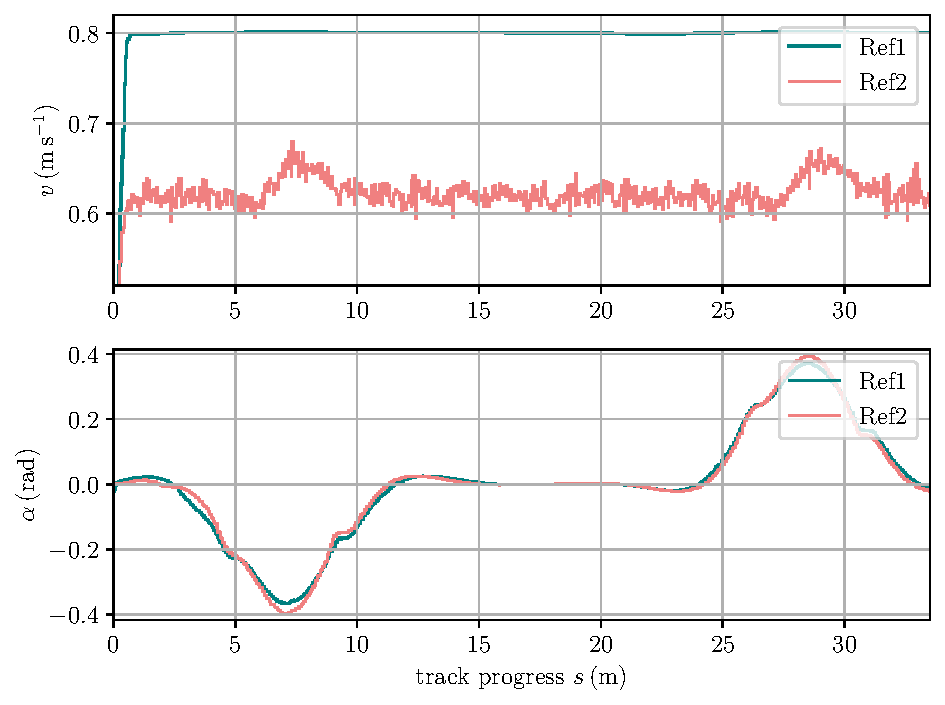
\includegraphics[width=1\textwidth]{figures/experiments/ucomp_ref}
\caption{Comparison of the impact of the application software's control thresholding for different reference trajectory schemes.} \label{fig_ucomp_ref}
\end{figure}
\begin{table}[h!tbp]
    \small
	\begin{center}
        \begin{tabular}{lccccl}\toprule
		    & \textbf{Ref1} & \textbf{Ref2}\\
            \midrule
            $\varepsilon_{v, \mathrm{osc}} $ & 4.26 $\cdot$ $10^{-3}$ $\mathrm{m\,s^{-1}}$& 2.59 $\cdot$ $10^{-2}$ $\mathrm{m\,s^{-1}}$\\
            $R$ & [ $5$, 2.5 $\cdot$ $10^{1}$ ] & [ $5$, 2.5 $\cdot$ $10^{1}$ ]\\
            $Q_{N}$ & [ $10^{-1}$, 2.5 $\cdot$ $10^{1}$, $10^{-8}$, $10^{-8}$, $5$ ] & [ $10^{-1}$, 2.5 $\cdot$ $10^{1}$, $10^{-8}$, $10^{-8}$, $5$ ]\\
            $Q$ & [ $10^{-8}$, 2.5 $\cdot$ $10^1$, $10^{-8}$, $10^{2}$, 10 ] & [ $10^{2}$, 2.5 $\cdot$ $10^1$, $10^{-8}$, $10^{-8}$ ] \\
		    \bottomrule
		\end{tabular}
	\end{center}
    \caption{Parameters of trajectory references with weighting matrices in SI units}
    \label{weight_ref}
\end{table}
The implicit velocity reference introduced Equation (\ref{eq_s_ref}) intended at progress maximization is unmerited in our case where the vehicles move on a dynamic warehouse floor, where time optimality does not take the highest priority. Instead, we introduce an explicit velocity reference in Equation (\ref{eq_v_ref}) only augmented by the former on the terminal shooting node to nudge the solution in the right direction at startup.
\par The superiority of the latter is seen in Figure \ref{fig_ucomp_ref} for this setup achieved by the state weights specified in Table \ref{weight_ref}. Another advantage of the explicit velocity reference is the geometric constraint simplification discussed in Section \ref{safety_field}.
\subsection{Delay compensation}\label{expr_del_comp}

\par Since the application layer is aware of the true applied input $\tilde{\zeta}^{u}$, unlike the MPC, three delay compensation schemes are investigated here for the round trip delay $\tau_{rt}$ as $\tau_{rt}$ = $\tau_{c}$ + $\tau_{a}$ + $\tau_{m}$. The first, referred to as $\mathrm{Eu}\,2$, relies on the delay compensation block in the application to account for $\tau_{m}$ + $\tau_{a}$, and the remaining delay compensation from the \ac{MPC} layer itself. In the second scheme i.e the $\mathrm{Eu}\,1$, the Euler predictor in the application compensates $\tau_{m}$, and $\tau_{c}$ + $\tau_{a}$ is compensated by forward simulating with the \ac{RK}4 integrator in the proposed controller. The third scheme, $\mathrm{Eu}\,0$ refers to complete $\tau_{rt}$ compensation in the \ac{MPC} layer. 

\begin{figure}[h!tbp]
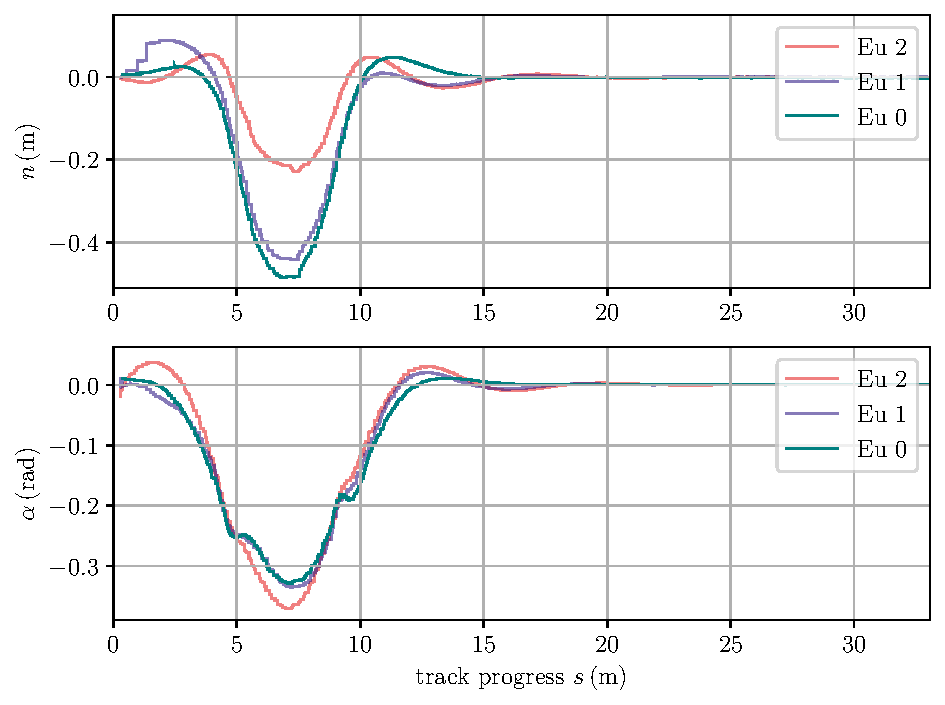
\includegraphics[width=1\textwidth]{figures/experiments/predictor}
\caption{Overshoot comparison of delay compensation schemes.}\label{fig1_comp_pred}
\end{figure}

\par After the right-hand curve on the track from $s$ = 7.5 m to $s$ = 10 m indicated in Figure \ref{test_track}, we see the decay of $n$ is marginally better with the $\mathrm{Eu}\,0$ in Figure \ref{fig1_comp_pred}. Despite the concern that the $\mathrm{Eu}\,0$ is agnostic to the applied vector $\tilde{\zeta^{u}}$ discussed in Section \ref{appr_oper_safe} that could lead to loss of solution robustness, the results discussed in Section \ref{comp_ref} with the explicit velocity reference assure us of the inactive control thresholding.
\par Thus, the sufficiency of the delay compensation purely in the \ac{MPC} layer is justified by experimental validation using the states $n$, $\alpha$.


\subsection{Direct and lifted formulations for the AGV elliptical footprint}

\begin{figure}[h!tb]
    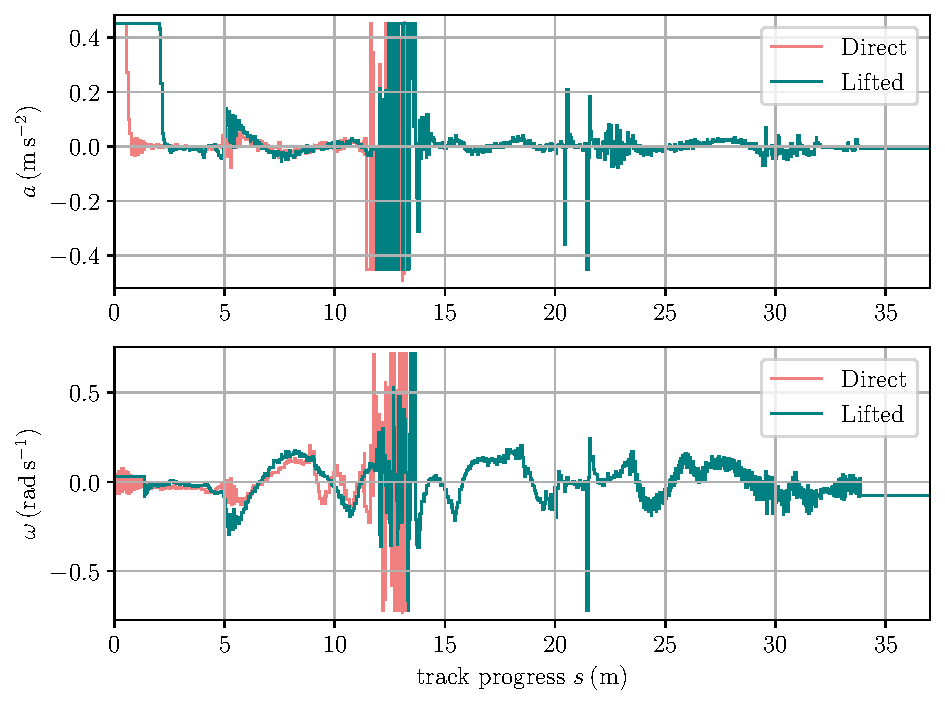
\includegraphics[width=1\textwidth]{figures/experiments/u_2c}
    \caption{Control $u$ comparison for the \ac{AGV} elliptical footprint and circular obstacles formulation in Gazebo.}  \label{fig_comp_u_2c}
\end{figure}

\begin{table}[h!tb]
    \small
	\begin{center}
        \begin{tabular}{lccccl}\toprule
		    & \textbf{Direct} & \textbf{Lifted}\\
            \midrule
            $\varepsilon_{a,\,\mathrm{osc}} $ & 7.95 $\cdot$ $10^{-1}\,\mathrm{m\,s^{-2}}$& 2.67 $\cdot$ $10^{-1}\,\mathrm{m\,s^{-2}}$\\
            $\varepsilon_{\omega,\,\mathrm{osc}} $ & 9.90 $\cdot$ $10^{-1}\,\mathrm{rad\,s^{-1}}$& 1.78 $\cdot$ $10^{-1}\,\mathrm{rad\,s^{-1}}$\\
		    \bottomrule
		\end{tabular}
	\end{center}
    \caption{Control oscillation metrics for the \ac{AGV} elliptical footprint and circular obstacles formulation in Gazebo.}
    \label{tab_u_osc_2c}
\end{table}

In this section, we inspect the solution trajectories of the \ac{OCP}s mentioned in Section \ref{appr_fren_traj} for the elliptical \ac{AGV} footprint. 
In order to achieve an unbiased comparison of the two trajectory tracking controllers with obstacle avoidance, we eliminate the drift of the obstacle state estimated by the \ac{KF} by assuming perfect knowledge of its position and dimensions.
As indicated previously in Section \ref{appr_footprint}, the elliptical \ac{AGV} footprint is a severely nonlinear function of the state $\zeta^{c}$, which can be seen in the poor convergence of the control trajectory $u$ in Figure \ref{fig_comp_u_2c}, for the direct elimination and lifted formulations.
Burdened with the additional nonlinearity introduced in the geometric constraint of the direct elimination formulation due to the nonlinear projection defined in Equation (\ref{F2C}), the simulated \ac{AGV} fails to maneuver around the first circular obstacle at $s$ = 13, where the solution stagnates at the poor local optima. Despite the lifted controller completing the track, we disqualify it from subsequent vehicle tests due to the poor quality of the controls. 

% \begin{figure}[h!tb]
%     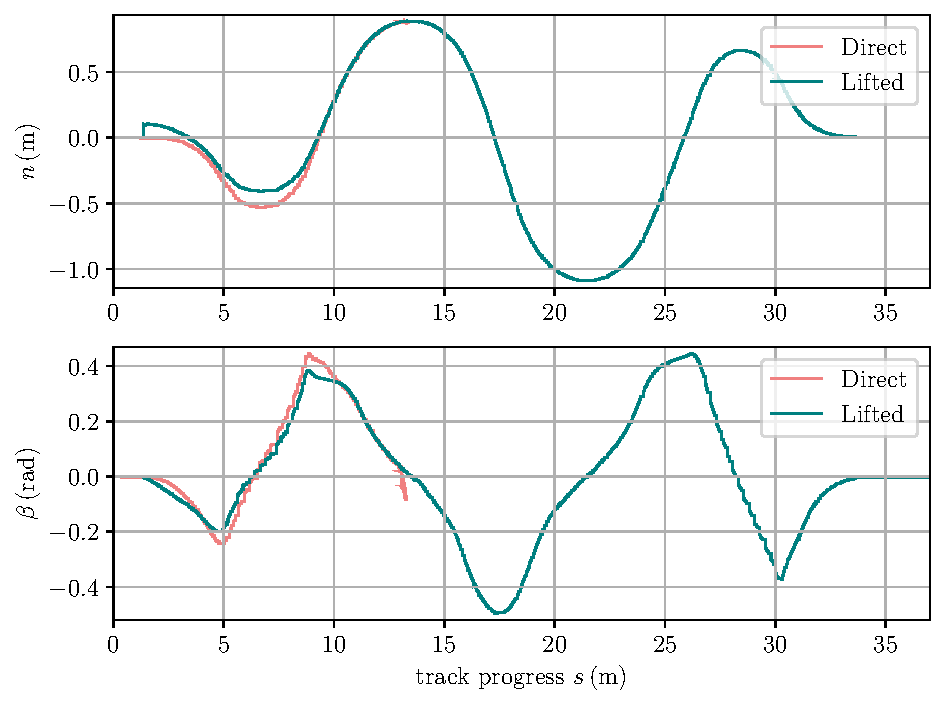
\includegraphics[width=1\textwidth]{figures/experiments/zeta_f_2c}
%     \caption{State $\zeta^{f}$ comparison from the closed loop Gazebo tests.}  \label{fig_comp_zeta_f}
% \end{figure}

\begin{figure}[h!tb]
    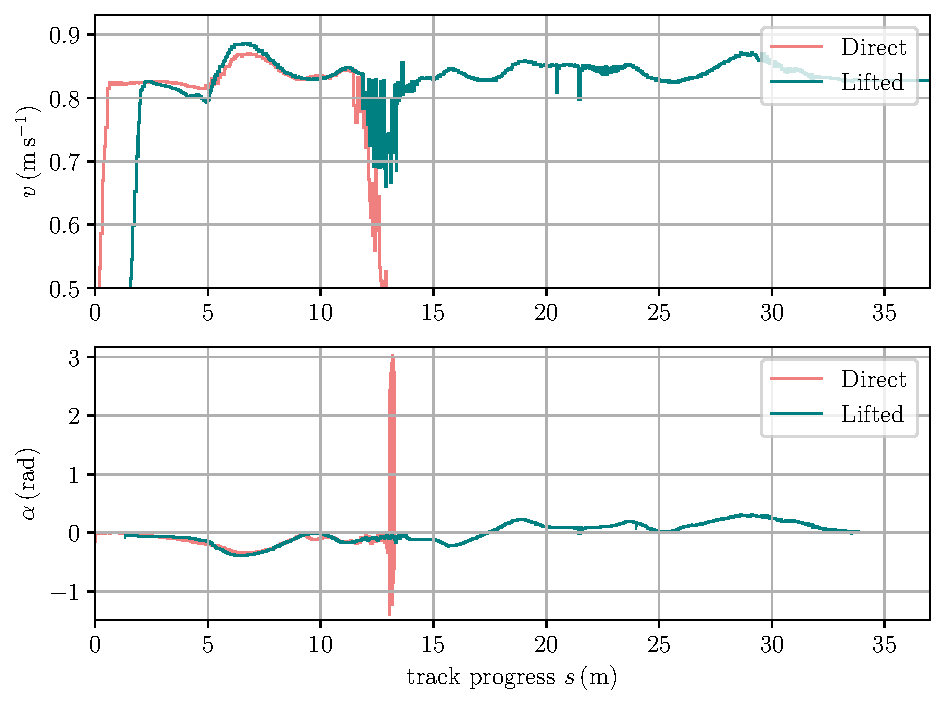
\includegraphics[width=1\textwidth]{figures/experiments/zeta_u_2c}
    \caption{State $\zeta^{u}$ comparison for the \ac{AGV} elliptical footprint and circular obstacles formulation in Gazebo.}  \label{fig_comp_zeta_u_2c}
\end{figure}

\begin{figure}[tb]
    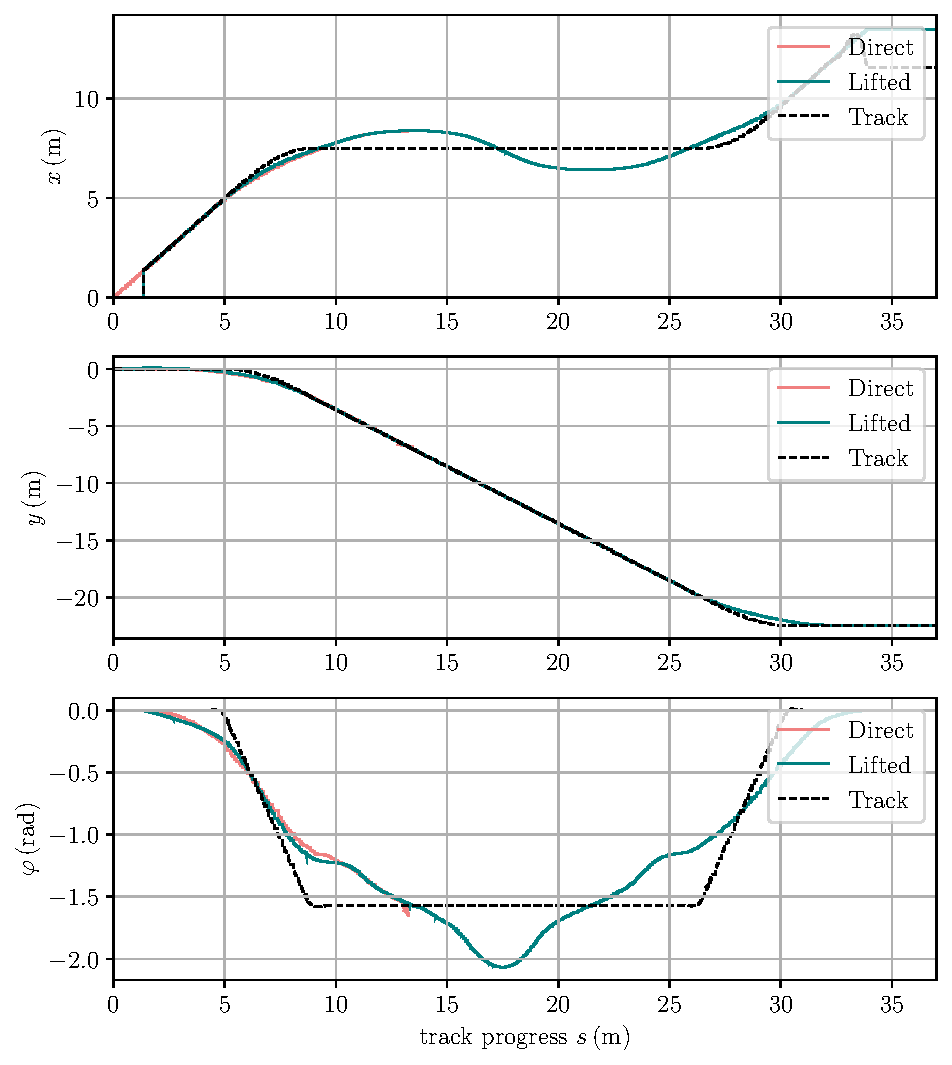
\includegraphics[width=1\textwidth]{figures/experiments/zeta_c_2c}
    \caption{State $\zeta^{c}$ comparison for the \ac{AGV} elliptical footprint and circular obstacles formulation in Gazebo.}  \label{fig_comp_zeta_c_2c}
\end{figure}
\newpage
% \newpage
\clearpage

\subsection{Direct and lifted formulations for the AGV covering circles}

\begin{figure}[h!tb]
    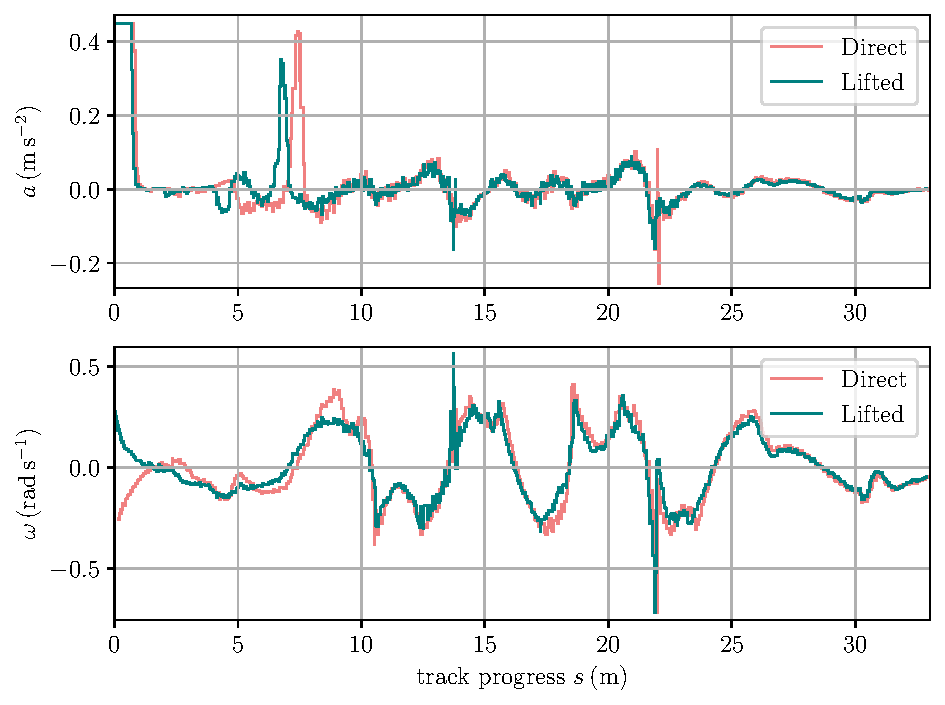
\includegraphics[width=1\textwidth]{figures/experiments/u}
    \caption{Control $u$ comparison for the \ac{AGV} covering circles and elliptical obstacles formulation in Gazebo.}  \label{fig_comp_u}
\end{figure}
\begin{table}[h!tb]
    \small
	\begin{center}
        \begin{tabular}{lccccl}\toprule
		    & \textbf{Direct} & \textbf{Lifted}\\
            \midrule
            $\varepsilon_{a,\,\mathrm{osc}} $ & 1.58 $\cdot$ $10^{-2}\,\mathrm{m\,s^{-2}}$& 1.56 $\cdot$ $10^{-2}\,\mathrm{m\,s^{-2}}$\\
            $\varepsilon_{\omega,\,\mathrm{osc}} $ & 1.57 $\cdot$ $10^{-2}\,\mathrm{rad\,s^{-1}}$& 2.25 $\cdot$ $10^{-2}\,\mathrm{rad\,s^{-1}}$\\
		    \bottomrule
		\end{tabular}
	\end{center}
    \caption{Control oscillation metrics for the \ac{AGV} covering circles and elliptical obstacles formulation in Gazebo.}
    \label{tab_u_osc_2el}
\end{table}

In this section, we proceed with the Gazebo tests for the covering circles, again under the assumption of no drift in the obstacle estimation. Observing the feasibility of both controllers for the task at hand, we carefully inspect the state and controls, with respect to the previously defined metrics.

\begin{figure}[h!tb]
    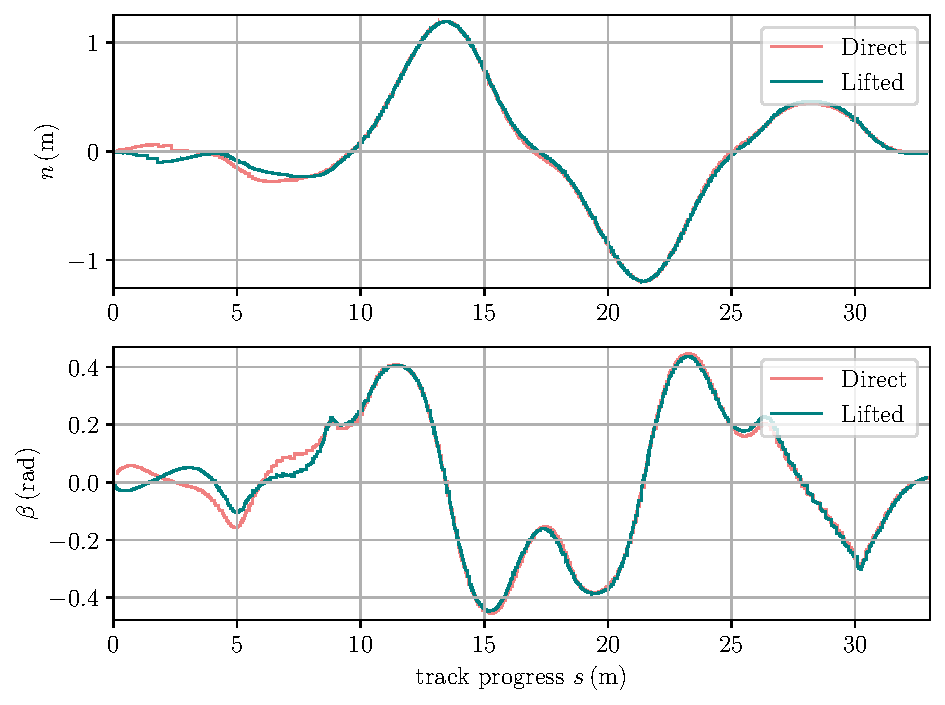
\includegraphics[width=1\textwidth]{figures/experiments/zeta_f}
    \caption{State $\zeta^{f}$ comparison for the \ac{AGV} covering circles and elliptical obstacles formulation in Gazebo.}  \label{fig_comp_zeta_f}
\end{figure}

\begin{figure}[h!tb]
    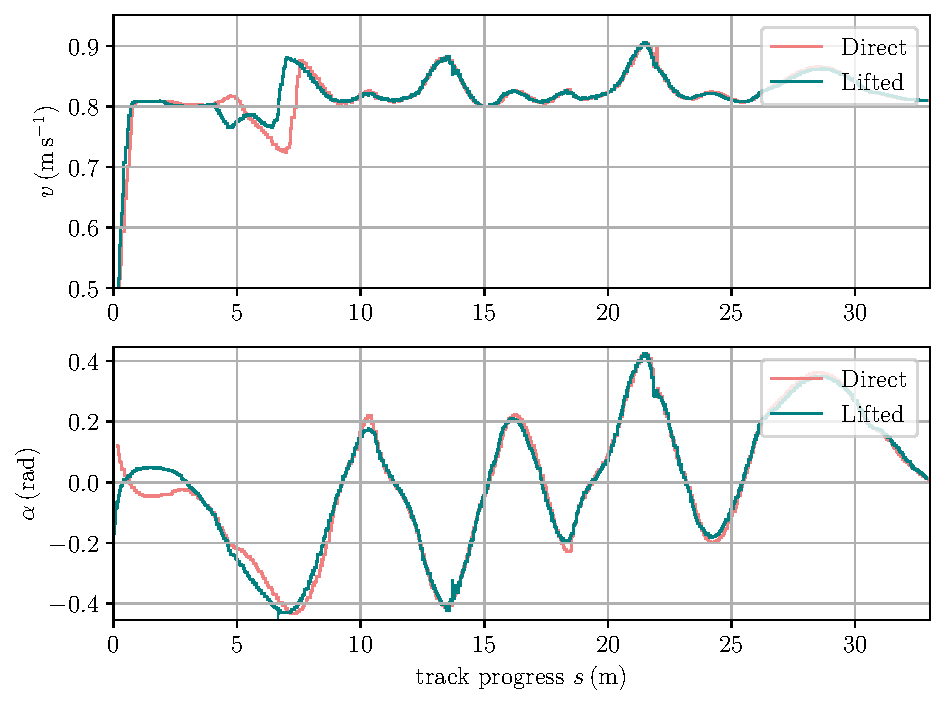
\includegraphics[width=1\textwidth]{figures/experiments/zeta_u}
    \caption{State $\zeta^{u}$ comparison for the \ac{AGV} covering circles and elliptical obstacles formulation in Gazebo.}  \label{fig_comp_zeta_u}
\end{figure}

\begin{figure}[h!tb]
    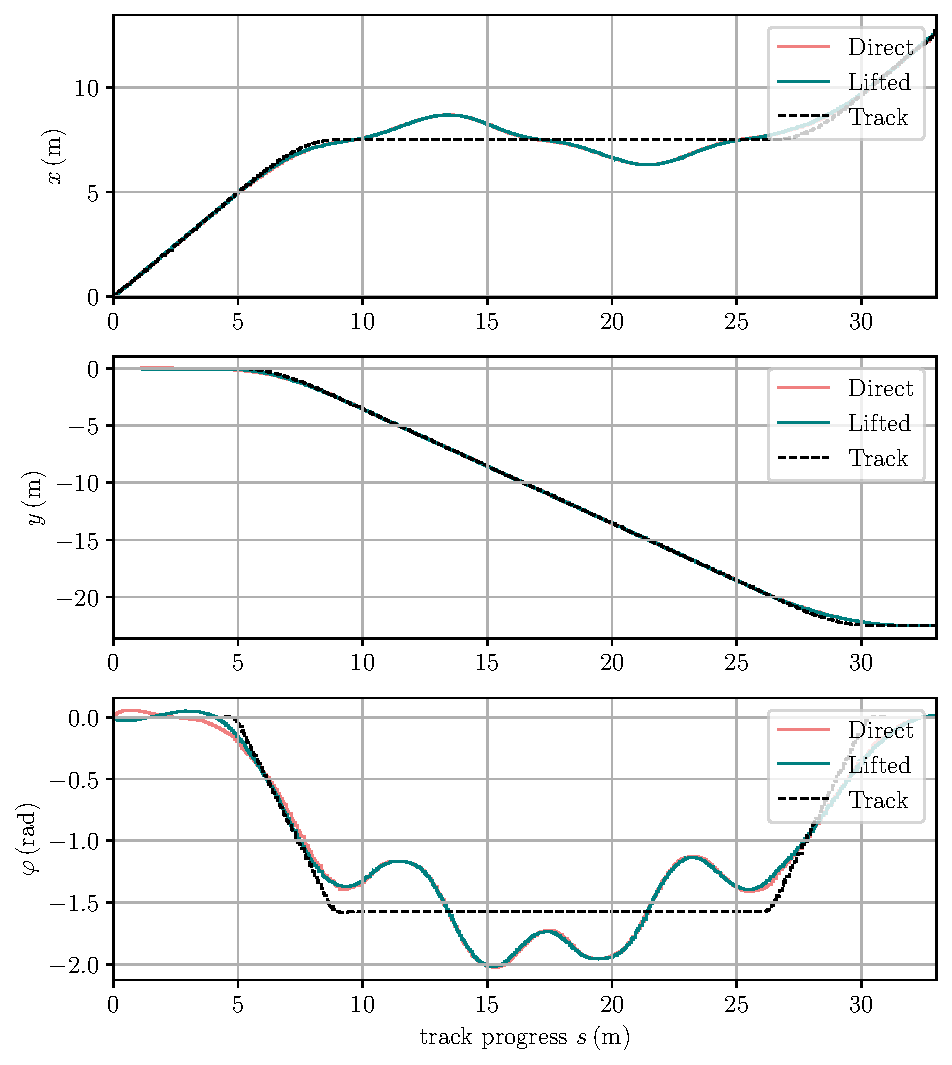
\includegraphics[width=1\textwidth]{figures/experiments/zeta_c}
    \caption{State $\zeta^{c}$ comparison for the \ac{AGV} covering circles and elliptical obstacles formulation in Gazebo.}  \label{fig_comp_zeta_c}
\end{figure}

\begin{figure}[h!tb]
    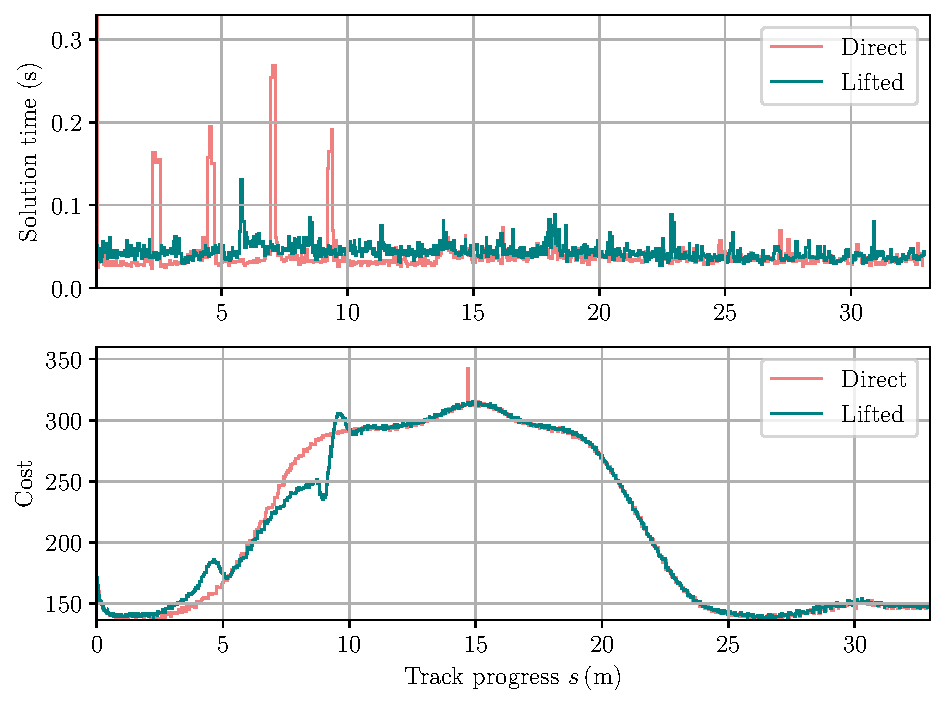
\includegraphics[width=1\textwidth]{figures/experiments/metrics}
    \caption{Solution comparison for the \ac{AGV} covering circles and elliptical obstacles formulation in Gazebo.}  \label{fig_metrics}
\end{figure}

\begin{table}[h!]
    \small
	\begin{center}
        \begin{tabular}{lccccl}\toprule
		    & \textbf{Direct} & \textbf{Lifted}\\
            \midrule
            $\varepsilon_{n,\,\mathrm{avg}} $ & 5.10 $\cdot$ $10^{-1}$ m& 5 $\cdot$ $10^{-1}$ m\\
            $\tau_{\mathrm{rti,\,avg}} $ & 3.99 $\cdot$ $10^{-2}$ s& 4.39 $\cdot$ $10^{-2}$ s\\
            $\tau_{\mathrm{rti,\,max}} $ & 2.69 $\cdot$ $10^{-1}$ s& 1.34 $\cdot$ $10^{-1}$ s\\
		    \bottomrule
		\end{tabular}
	\end{center}
    \caption{Centreline deviation and solution times for the \ac{AGV} covering circles and elliptical obstacles formulation in Gazebo.}
    \label{tab_rti_sim}
\end{table}

Both formulations tested here complete the track with similar solution trajectories as indicated in Figures \ref{fig_comp_zeta_c}, \ref{fig_comp_zeta_f}, \ref{fig_comp_zeta_u}, and \ref{fig_comp_u} with minor differences in solution times. These differences, however, are significant in evaluating real-time feasibility of the proposed optimal control schemes. In Figure \ref{fig_metrics}, we observe that, although the direct elimination formulation has a lower average SQP solution time $\tau_{\mathrm{rti,\,avg}}$, it exceeds the MPC assigned computation deadline $\tau_{c}$ several times. Since the drive controller applies the previous control in this scenario, the guarantee of overall solution optimality is lost, despite retaining the feasibility of the trajectory tracking problem.
\goodbreak
\newpage
% \newpage
\clearpage

\section{Warehouse tests}

Both formulations are tested with cylindrical and cuboidal obstacles, with the \ac{AGV} covering circles formulation along the track at the warehouse, similar to the one previously described in the Gazebo simulation. The track begins with a right-hand curve followed by a $20 \mathrm{m}$ long straight path and ends with a left curve. The obstacles are placed at $s$ = $13 \mathrm{m}$ and $s$ = $17\mathrm{m}$ offset by $n$ = $0.25 \mathrm{m}$ and $n$ = $-0.25 \mathrm{m}$ respectively from the centre line. The unreliability of obstacle detection with the laser scanner's limited field of view aboard the \ac{AGV} is further exacerbated by the need to exclude vehicle chassis reflections. To avoid the \ac{AGV} footprint being considered as an active constraint, leading to infeasibility, a minimal angle is used in conjunction with the \ac{KF} to estimate the occluded objects during maneuvres. The closed-loop trajectories of state and control of the lifted formulation are presented in Figures \ref{fig_zeta_time} and \ref{fig_u_time}.
\par We continue to use the RTI scheme as in simulation, to solve the \ac{OCP}s aboard the \ac{AGV}, which is equipped with an industrial computer running the \ac{ROS} Noetic framework for Ubuntu on an Intel i7 9700TE @ 1.8 Ghz. The $\tau_{\mathrm{rti,\,avg}}$ indicates that the solution times are well within the soft deadline $\tau_{c}$ of the MPC node during the remainder of the tracking, proving its feasibility. Additionally, comparing the obtained SQP solution times in Tables \ref{tab_rti_sim} and \ref{tab_rti_agv}, the lower average SQP solution times for both formulations on the vehicle strengthens the argument that the lifted formulation is en route to real-time optimal performance.
\begin{figure}[h!tb]
    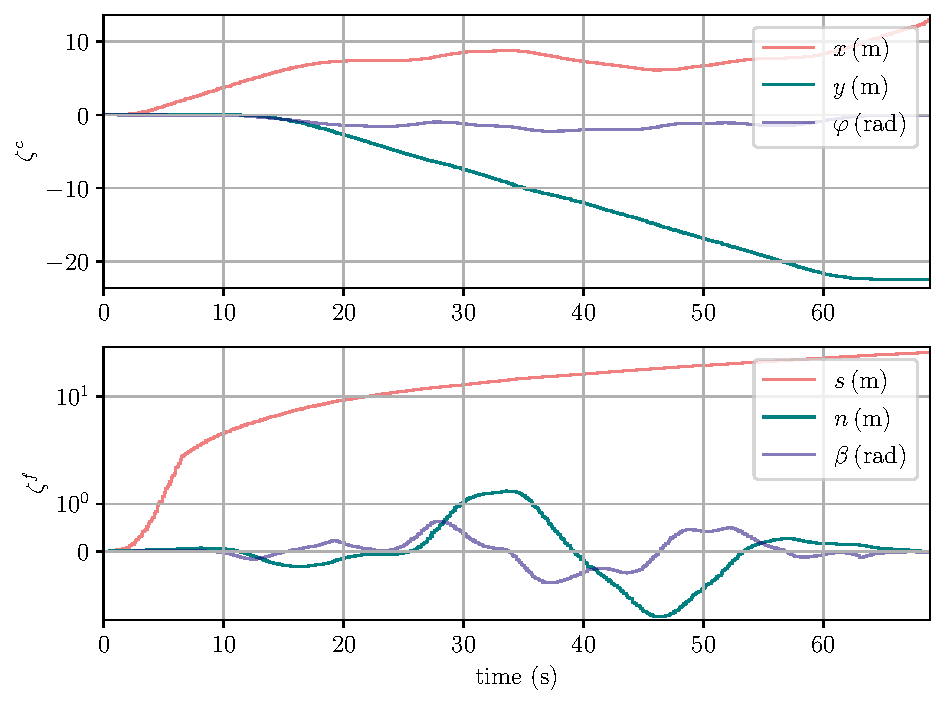
\includegraphics[width=1\textwidth]{figures/experiments/zeta_time}
    \caption{State $\zeta^{l}$ for the lifted formulation with \ac{AGV} covering circles and elliptical obstacles from the real warehouse.}  \label{fig_zeta_time}
\end{figure}
\begin{table}[tb]
    \small
	\begin{center}
        \begin{tabular}{lccccl}\toprule
		    & \textbf{Direct} & \textbf{Lifted}\\
            \midrule
            $\varepsilon_{n, \mathrm{avg}} $ & 3.828 $\cdot$ $10^{-1}$ m& 4.688 $\cdot$ $10^{-1}$ m\\
            $\tau_{\mathrm{rti,\,avg}} $ & 2.899 $\cdot$ $10^{-2}$ s& 3.099 $\cdot$ $10^{-2}$ s\\
		    \bottomrule
		\end{tabular}
	\end{center}
    \caption{Centreline deviation and average solution time for the \ac{AGV} covering circles and elliptical obstacles formulation in the real warehouse.}
    \label{tab_rti_agv}
\end{table}
\begin{table}[h!]
    \small
	\begin{center}
        \begin{tabular}{lccccl}\toprule
		    & \textbf{Direct} & \textbf{Lifted}\\
            \midrule
            $\varepsilon_{v,\,\mathrm{osc}} $ & 7.96 $\cdot$ $10^{-2}\,\mathrm{m\,s^{-1}}$& 4.37 $\cdot$ $10^{-2}\,\mathrm{m\,s^{-1}}$\\
            $\varepsilon_{a,\,\mathrm{osc}} $ & 5.69 $\cdot$ $10^{-2}\,\mathrm{m\,s^{-2}}$& 9.52 $\cdot$ $10^{-2}\,\mathrm{m\,s^{-2}}$\\
            $\varepsilon_{\omega,\,\mathrm{osc}} $ & 1.66 $\cdot$ $10^{-1}\,\mathrm{rad\,s^{-1}}$& 2.86 $\cdot$ $10^{-1}\,\mathrm{rad\,s^{-1}}$\\
		    \bottomrule
		\end{tabular}
	\end{center}
    \caption{Control oscillation metrics for the \ac{AGV} covering circles and elliptical obstacles formulation in the real warehouse.}
    \label{tab_u_osc_agv_2el}
\end{table}
\begin{figure}[h!]
    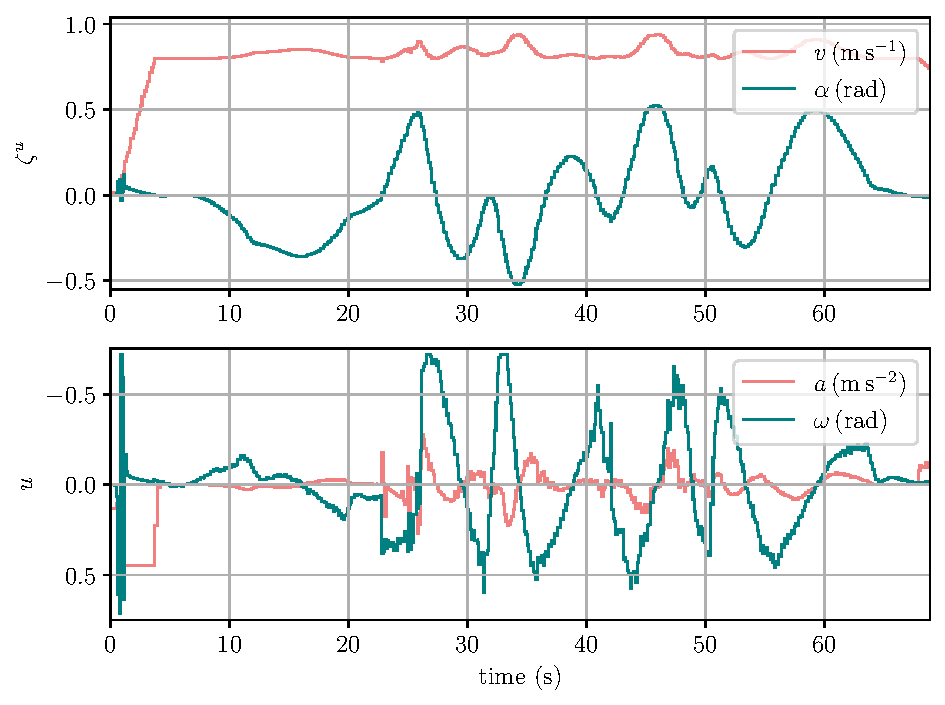
\includegraphics[width=1\textwidth]{figures/experiments/u_time}
    \caption{Control $u$ for the the lifted formulation with \ac{AGV} covering circles and elliptical obstacles from the real warehouse.}  \label{fig_u_time}
\end{figure}
    \chapter{Conclusion}\label{chap:conclusion}

The optimal controllers designed in this work have been experimentally validated for real-time performance, proving their feasibility for tricycle kinematic \ac{AGV}s in a warehouse environment. By demonstrating the real-time feasibility of acados for NMPC, the groundwork for the motion control scheme has been laid, paving the way for its extension to production vehicles with various kinematic models.
\par This work highlights a methodical approach to implement two optimal control schemes on an industrial vehicle.
A significant effort is spent investigating and developing the appropriate model for the task, motivated by physical motion constraints and safety mechanisms.    
Starting with IPOPT to validate the control scheme, we then proceed to use acados to achieve the closed loop control in a time and computation-bound environment.
In order to realistically gauge the control performance, we progress to a higher fidelity model in Gazebo, by incorporating the \ac{MPC} node into ek robotics' application software. This involves appropriately utilizing the state feedback from wheel encoders, and localization data from the onboard \ac{SLAM} stack to design a suitable state observer and delay compensation scheme.
\par With a feasible trajectory tracking scheme verified in the real warehouse, we then proceed to conservative constraint formulations for the large \ac{AGV} footprint, considering approximations of real obstacles in the test environment. This not only involves selecting an open-source obstacle detector and abstracting laser scan data to handle multiple objects, but also identifying and using an appropriate estimator to provide obstacle predictions for occluded objects. Finally, we compare the obstacle constraint formulations and controller performance in Gazebo and on the real vehicle \ac{AGV}.
\par The two controllers exhibit similar performance for the AGV covering circles, but the lifted Frenet indicates better performance for the more nonlinear formulation, in the elliptical footprint, highlighting its improved constraint handling.
\par Obtaining more rigorous guarantees on obstacle avoidance, however, calls for a more rugged obstacle detection mechanism that can provide a full field of view among others. Another foreseen improvement is that; the simplified obstacle constraints introduced in the Cartesian frame could further be extended to more generic convex polygons, better representing the working environment of such vehicles. 
    \chapter{Acknowledgments}

I would like to utilize this section to thank the University of Freiburg and ek robotics for the opportunity to apply the theoretical knowledge obtained in the course of my Master's, through this thesis. Acknowledging the policy of unrestricted access to cutting-edge research at the Chair of Systems Optimization and Control headed by Prof. Dr. Moritz Diehl, I would like to thank Jonathan Frey for his careful supervision and innovative proposals. A word of thanks is due to Rudolf Reiter for his constructive feedback, Wim Van Roy and several other team members at the department, with whom I could freely brainstorm. The exchange of views with my fellow students, Yizhen Wang, Mohammed Hababeh and Sourish Pramanick often provided new perspectives in the face of stubborn challenges. 
\par At ek robotics, I would like to especially mention the team of Karsten Bohlmann, starting with Kathrin Pregizer and Peter Götz, whose timely ideas for practical constraints went a long way in realizing the experiments. Daniel Klöser who facilitated this collaboration, has been an exemplary advisor whose patience and meticulous direction have been invaluable from ideation to execution. I am also thankful for friends and family whose encouragement kept me motivated and in good cheer, and God almighty for the strength to see this through.
  
     
    \bibliographystyle{ieeetr}
    \bibliography{./syscop_bibtex/thesis.bib}
    \addcontentsline{toc}{chapter}{Bibliography}
    \newpage



\end{document}
